\documentclass[a4paper,12pt]{article}
\usepackage{indentfirst}
\usepackage[T1]{fontenc}
\usepackage{graphicx}
\usepackage{booktabs}
\usepackage{array}
\usepackage{tabularx}
\usepackage{float}
\usepackage{caption}
\usepackage{subcaption}
\graphicspath{{../Imagens/}{Imagens/}}
\renewcommand{\figurename}{Figura}
\renewcommand{\tablename}{Tabela}
\captionsetup{
  justification=raggedright,
  singlelinecheck=false,
  labelsep=endash,
  font=small,
  labelfont=bf,
  skip=6pt
}
\captionsetup[figure]{position=above}
\captionsetup[table]{position=above}
\newfloat{quadro}{htbp}{loq}
\floatname{quadro}{Quadro}
\captionsetup[quadro]{position=above}
\newcommand{\fonteelemento}[1]{%
  \par\smallskip
  {\footnotesize\raggedright Fonte: #1.\par}%
}

\begin{document}

\section{Resultados e Discuss\~ao}


Este cap\'itulo re\'une os resultados atualmente documentados sobre a plataforma e discute seu alcance.


O firmware integrado, o caderno de ensaios, as fotografias dos instrumentos dispon\'iveis, os relat\'orios de compila\c{c}\~ao e as figuras dos resultados funcionais foram incorporados ao reposit\'orio. A montagem provis\'oria foi documentada por descri\c{c}\~ao e mapa de liga\c{c}\~oes, sem fotografia panor\^amica adicional.

Extensibilidade e acoplamento foram avaliados estruturalmente; a mem\'oria global foi medida; a inicializa\c{c}\~ao degradada foi verificada qualitativamente; e os testes funcionais dos sensores, RTC, consumo de corrente e condicionamento PPG foram incorporados. Permaneceram fora do escopo final a mem\'oria incremental por m\'odulo, CPU e heap por cen\'ario e a efic\'acia din\^amica da recupera\c{c}\~ao I$^2$C sob falha induzida, limita\c{c}\~oes explicitadas nas se\c{c}\~oes correspondentes.


\subsection{Estado das evid\^encias}


Para evitar atribuir a mesma for\c{c}a a registros distintos, as evid\^encias foram classificadas nos tr\^es n\'iveis apresentados no Quadro~\ref{qua:niveis-evidencia}.


\begin{quadro}[H]
\centering
\caption{Classifica\c{c}\~ao das evid\^encias empregadas}
\label{qua:niveis-evidencia}
\small
\begin{tabularx}{\textwidth}{|>{\raggedright\arraybackslash}p{0.20\textwidth}|>{\raggedright\arraybackslash}p{0.34\textwidth}|>{\raggedright\arraybackslash}X|}
\hline
\textbf{N\'ivel} & \textbf{Descri\c{c}\~ao} & \textbf{Uso neste cap\'itulo} \\
\hline
evid\^encia prim\'aria & firmware, log, tabela, s\'erie temporal, fotografia ou arquivo de ensaio dispon\'ivel & base para resultado reproduz\'ivel \\
\hline
registro consolidado & valor resumido nos documentos de controle ou nos compilados, sem dado prim\'ario dispon\'ivel & resultado provis\'orio a conferir \\
\hline
observa\c{c}\~ao funcional & relato de bancada sem procedimento completo, instrumento identificado ou repeti\c{c}\~oes & demonstra funcionamento, n\~ao desempenho quantitativo \\
\hline
\end{tabularx}
\fonteelemento{Elaborado pelo autor}
\end{quadro}


O caderno de ensaios e as figuras associadas fornecem evid\^encias prim\'arias para os testes funcionais dos sensores, do RTC e do consumo de corrente. Os resultados arquiteturais permanecem predominantemente apoiados na implementa\c{c}\~ao e em registros consolidados.


\subsection{Prot\'otipo integrado}


Os documentos de consolida\c{c}\~ao descrevem um prot\'otipo formado pelo XIAO ESP32-C6 encaixado no Round Display e por quatro unidades sensoriais externas: MAX30102, DS18B20, LTR390 e MPU-9250/AK8963. A interface inclui tela principal, navega\c{c}\~ao por toque e telas dedicadas \`as fun\c{c}\~oes. O RTC PCF8563 mant\'em data e hora.


A integra\c{c}\~ao combina SPI2 para o display, I$^2$C compartilhado para toque, RTC e sensores e 1-Wire por RMT para temperatura. Esse conjunto demonstra funcionalmente que a plataforma comporta dispositivos com transportes e ciclos de aquisi\c{c}\~ao diferentes.


A fotografia da placa em opera\c{c}\~ao, as renderiza\c{c}\~oes e o mapa de liga\c{c}\~oes foram apresentados em Materiais e M\'etodos. N\~ao se repete aqui a mesma evid\^encia visual, pois a configura\c{c}\~ao sensorial avaliada corresponde \`aquela montagem.


\subsection{Cumprimento dos requisitos}


A s\'intese do Quadro~\ref{qua:estado-requisitos} separa implementa\c{c}\~ao confirmada, teste funcional e limita\c{c}\~ao de avalia\c{c}\~ao.


\begin{quadro}[H]
\centering
\caption{Estado dos requisitos da plataforma}
\label{qua:estado-requisitos}
\small
\begin{tabularx}{\textwidth}{|>{\raggedright\arraybackslash}p{0.23\textwidth}|>{\raggedright\arraybackslash}p{0.25\textwidth}|>{\raggedright\arraybackslash}X|}
\hline
\textbf{Requisito} & \textbf{Estado documentado} & \textbf{Evid\^encia dispon\'ivel} \\
\hline
contrato de m\'odulos & implementado & descri\c{c}\~ao consolidada de inicializa\c{c}\~ao, cria\c{c}\~ao e exibi\c{c}\~ao de tela \\
\hline
integra\c{c}\~ao dos sensores & testada funcionalmente & caderno de ensaios, tabelas e figuras dos m\'odulos \\
\hline
navega\c{c}\~ao por toque & testada funcionalmente & compilado do Round Display e resumo consolidado \\
\hline
compartilhamento do I$^2$C & implementado & mapa consolidado, mutex e servi\c{c}o de recupera\c{c}\~ao descritos \\
\hline
inicializa\c{c}\~ao n\~ao fatal & implementada & descri\c{c}\~ao arquitetural \\
\hline
extensibilidade & prevista e implementada arquiteturalmente & contrato e pontos de registro descritos \\
\hline
toler\^ancia a falhas & mecanismos implementados & inicializa\c{c}\~ao n\~ao fatal e recupera\c{c}\~ao p\'os-NACK descritas \\
\hline
uso de recursos & parcialmente registrado & tamanho integrado e pool do LVGL nos documentos \\
\hline
fun\c{c}\~oes sensoriais & testadas funcionalmente & compara\c{c}\~oes funcionais e ensaios controlados registrados \\
\hline
\end{tabularx}
\fonteelemento{Elaborado pelo autor a partir do firmware e do caderno de ensaios}
\end{quadro}


O quadro permite afirmar que a arquitetura e os m\'odulos foram implementados, mas n\~ao que todos os objetivos de avalia\c{c}\~ao tenham sido cumpridos. Extensibilidade e acoplamento receberam uma avalia\c{c}\~ao estrutural retrospectiva; recursos computacionais e robustez din\^amica permanecem abertos.


\subsection{Arquitetura modular}


\subsubsection{Contrato dos m\'odulos}


Os registros indicam que MAX30102, DS18B20, LTR390 e as fun\c{c}\~oes baseadas no MPU-9250 foram integrados pelo mesmo ciclo de vida: inicializa\c{c}\~ao, cria\c{c}\~ao da tela e exibi\c{c}\~ao. O n\'ucleo registra telas e atualiza\c{c}\~oes, enquanto os algoritmos permanecem nos m\'odulos. O DS18B20 utiliza 1-Wire sem obrigar os demais componentes a conhecer esse transporte.


Essa evid\^encia \'e estrutural e mostra a presen\c{c}a de um ponto comum de integra\c{c}\~ao.

A confer\^encia do firmware mostrou que cada tela sensorial inclui \texttt{app.h} para registrar sua fun\c{c}\~ao de atualiza\c{c}\~ao. Os m\'odulos mant\^em estado em vari\'aveis est\'aticas locais ao arquivo e n\~ao acessam diretamente o estado de outros sensores. O n\'ucleo, entretanto, conhece explicitamente os cabe\c{c}alhos e os pontos de entrada de cada m\'odulo; a composi\c{c}\~ao n\~ao \'e din\^amica.


\subsubsection{Esfor\c{c}o de adi\c{c}\~ao de m\'odulo}

Como n\~ao foi integrado um componente novo durante a fase de avalia\c{c}\~ao, foi realizado um estudo retrospectivo do MAX30102. O projeto standalone possui 1307 linhas distribu\'idas em nove arquivos C e H; o m\'odulo integrado possui 1315 linhas em dez arquivos. Os seis arquivos de processamento \texttt{heart\_rate.c/.h}, \texttt{ppg\_filter.c/.h} e \texttt{spo2.c/.h}, totalizando 678 linhas, s\~ao id\^enticos nas duas vers\~oes.

O driver de hardware foi modificado para receber o barramento e o mutex compartilhados, recuperar o I$^2$C ap\'os erro e permitir ativa\c{c}\~ao e desligamento da aquisi\c{c}\~ao. As 294 linhas do \texttt{main.c} standalone foram substitu\'idas por 331 linhas em \texttt{max30102\_screen.c/.h}, que concentram tarefa, estado, callbacks, tela e interface p\'ublica. N\~ao foram encontradas altera\c{c}\~oes em outros m\'odulos sensoriais.

A integra\c{c}\~ao deixou seis pontos expl\'icitos fora da pasta do MAX30102: inclus\~ao do cabe\c{c}alho, callback de exibi\c{c}\~ao, item de menu, inicializa\c{c}\~ao, cria\c{c}\~ao da tela e diret\'orio de inclus\~ao no CMake. Assim, a estrutura concentra as mudan\c{c}as e preserva o processamento, mas n\~ao elimina edi\c{c}\~oes no n\'ucleo. Como o levantamento foi posterior \`a implementa\c{c}\~ao e n\~ao preservou o tempo de trabalho, ele caracteriza a estrutura da mudan\c{c}a, n\~ao o esfor\c{c}o temporal.


\subsubsection{Acoplamento e altera\c{c}\~oes no n\'ucleo}

A an\'alise dos cabe\c{c}alhos n\~ao encontrou depend\^encias diretas entre MAX30102, DS18B20 e LTR390. O ped\^ometro depende intencionalmente de \texttt{mpu9250\_hw}, pois reutiliza o aceler\^ometro da mesma unidade inercial. MAX30102, LTR390, MPU-9250 e RTC dependem do servi\c{c}o de recupera\c{c}\~ao do I$^2$C; o DS18B20 permanece fora desse barramento.

N\~ao foi identificado ciclo direto no grafo de inclus\~ao de cabe\c{c}alhos. No n\'ivel de pacotes existe uma depend\^encia bidirecional controlada: o n\'ucleo inclui as interfaces dos m\'odulos para comp\^o-los, enquanto as telas usam o contrato de \texttt{app.h} para registrar callbacks e obter servi\c{c}os comuns. Esse resultado \'e mais preciso do que classificar a arquitetura inteira como estritamente ac\'iclica. A Figura~\ref{fig:dependencias-firmware} apresenta o grafo obtido.

\begin{figure}[H]
\centering
\caption{Depend\^encias identificadas por an\'alise est\'atica do firmware integrado}
\label{fig:dependencias-firmware}
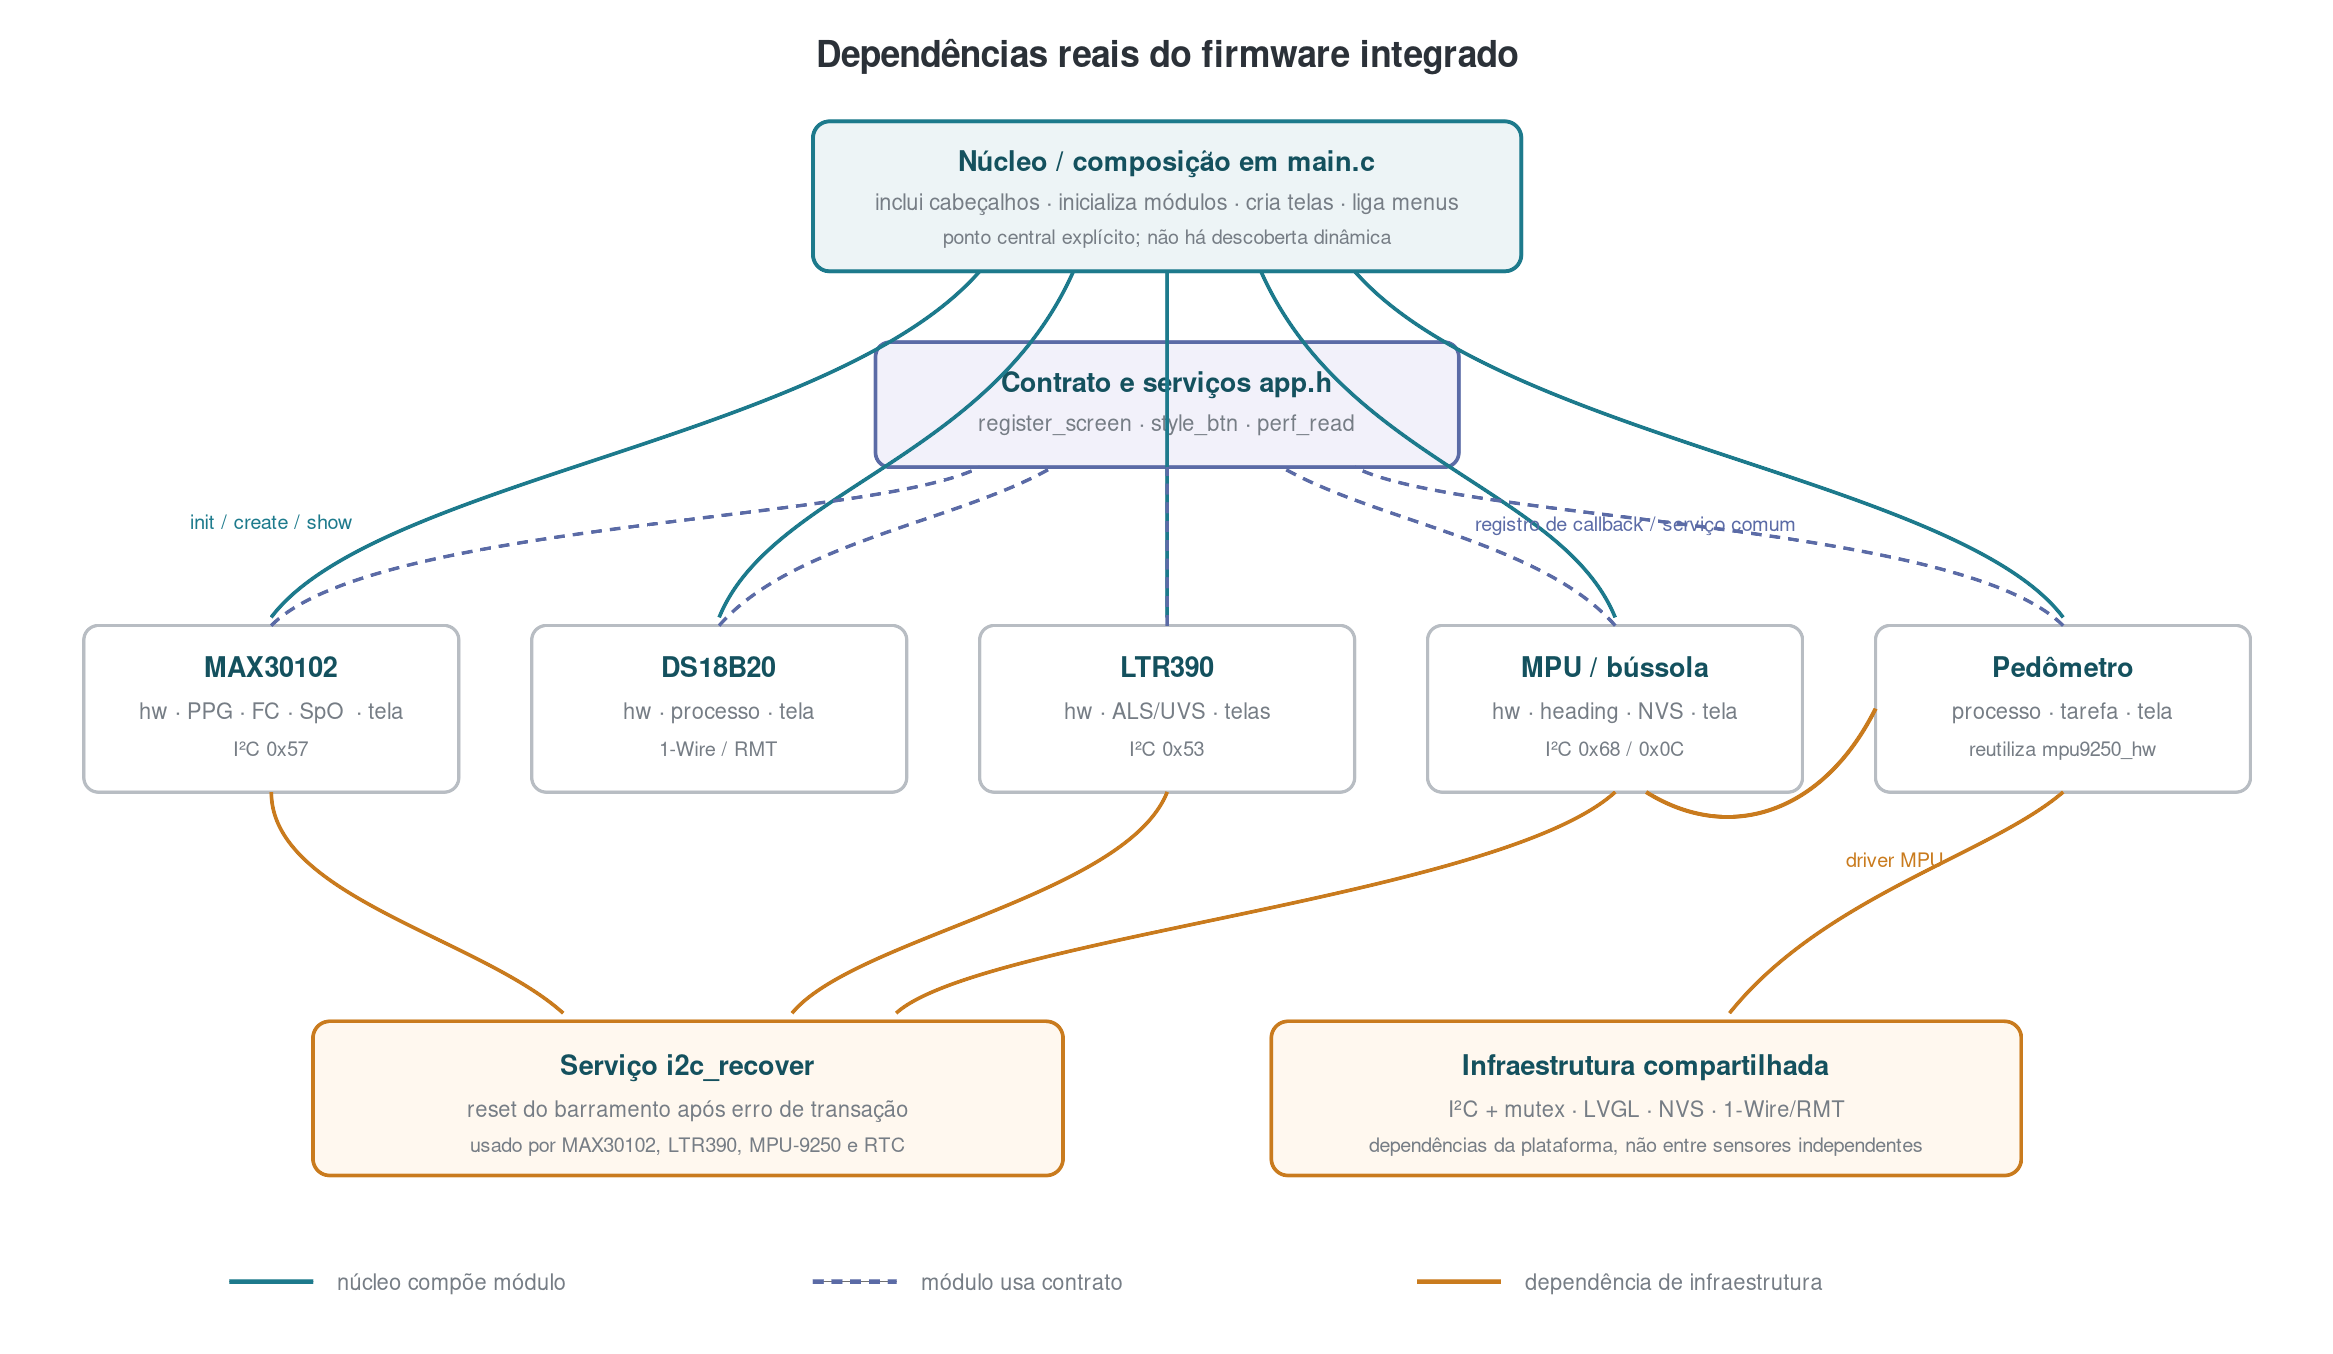
\includegraphics[width=0.98\textwidth]{Diagramas/sistema/dependencias_firmware.png}
\fonteelemento{Elaborado pelo autor a partir das inclus\~oes e chamadas do firmware}
\end{figure}


\subsection{Recursos computacionais}


\subsubsection{Tamanho do bin\'ario}


A vers\~ao final do bin\'ario avaliado foi obtida por uma compila\c{c}\~ao limpa e analisada com as ferramentas \texttt{size} e \texttt{size-components} do ESP-IDF v5.5.1.


O arquivo grav\'avel apresentou 784.240 bytes (765,86 KiB) em uma parti\c{c}\~ao de 1.048.576 bytes (1.024 KiB). Isso corresponde a 74,79\% de ocupa\c{c}\~ao e 264.336 bytes (258,14 KiB, ou 25,21\%) de folga; a sa\'ida resumida do ESP-IDF apresenta 25\%. A ferramenta \texttt{size} reportou imagem de 784.124 bytes, 116 bytes menor que o arquivo devido ao preenchimento do bin\'ario. O resultado confirma a ordem de grandeza anteriormente descrita como aproximadamente 760 KiB. A compara\c{c}\~ao com o registro anterior de 643 KB, contudo, n\~ao permite atribuir a diferen\c{c}a aos sensores, pois as vers\~oes podem diferir em fontes, componentes, otimiza\c{c}\~ao e recursos gr\'aficos.

Os relat\'orios completos de \texttt{size} e \texttt{size-components} foram preservados com os demais registros de an\'alise do trabalho.


\subsubsection{Mem\'oria por m\'odulo e heap}


O pool interno do LVGL foi configurado para 96 KiB depois que 32 KiB se mostraram insuficientes para criar os objetos da b\'ussola. Essa altera\c{c}\~ao documenta uma restri\c{c}\~ao de integra\c{c}\~ao.

O relat\'orio est\'atico registrou 179.360 bytes de DIRAM utilizados em 452.112 bytes considerados pela ferramenta, ou 39,67\%, com 272.752 bytes remanescentes. O total utilizado reuniu 105.632 bytes de BSS, 65.512 bytes de c\'odigo em DIRAM e 8.216 bytes de dados inicializados. Para flash, foram registrados 710.364 bytes de c\'odigo e constantes. No relat\'orio por bibliotecas, o LVGL respondeu por 361.202 bytes de contribui\c{c}\~ao ao ELF, incluindo 99.460 bytes de BSS, enquanto \texttt{libmain.a} reuniu 207.325 bytes. Esses valores de biblioteca n\~ao representam incrementos isolados dos sensores, e a DIRAM remanescente no mapa n\~ao equivale ao heap livre durante a execu\c{c}\~ao.


N\~ao foram executadas compila\c{c}\~oes incrementais nem coletas de heap por cen\'ario. Por isso, n\~ao se apresenta uma decomposi\c{c}\~ao gr\'afica por m\'odulo: produzi-la a partir do relat\'orio integrado atribuiria custos que os dados n\~ao permitem isolar.


\subsubsection{CPU e tempo de boot}

A ocupa\c{c}\~ao de CPU e o heap din\^amico n\~ao foram medidos de forma compar\'avel entre cen\'arios. A inspe\c{c}\~ao mostrou que \texttt{app\_perf\_read()} era chamada somente pela tela principal e comparava deltas do contador ocioso sem normalizar intervalos transcorridos quando outras telas permaneciam ativas. Os relat\'orios de compila\c{c}\~ao quantificam flash e mem\'oria est\'atica, mas n\~ao substituem medi\c{c}\~oes de CPU ou heap em execu\c{c}\~ao. Por isso, n\~ao se apresenta percentual de CPU nem se mant\'em a afirma\c{c}\~ao hist\'orica de carga inferior a 1\%.

Os tempos de boot dispon\'iveis pertencem ao piloto de inicializa\c{c}\~ao degradada descrito adiante. Como houve uma execu\c{c}\~ao registrada por condi\c{c}\~ao, os valores caracterizam os casos observados e n\~ao uma distribui\c{c}\~ao estat\'istica do tempo de inicializa\c{c}\~ao.


\subsection{Robustez e estabilidade}


\subsubsection{NACK e recupera\c{c}\~ao}


Os registros de desenvolvimento descrevem a implementa\c{c}\~ao de \texttt{i2c\_master\_bus\_\allowbreak reset()} ap\'os falhas e a remo\c{c}\~ao de uma opera\c{c}\~ao de \texttt{SW\_RESET} do LTR390 que produzia NACK previs\'ivel. Um erro de um m\'odulo foi, portanto, tratado como problema sist\^emico do recurso compartilhado.

A an\'alise est\'atica confirmou que os caminhos de erro dos drivers I$^2$C chamam o servi\c{c}o de recupera\c{c}\~ao antes de devolver o resultado da transa\c{c}\~ao. Essa evid\^encia demonstra a presen\c{c}a e a integra\c{c}\~ao do mecanismo no c\'odigo, mas n\~ao mede sua taxa de sucesso, sua lat\^encia nem a continuidade dos demais endere\c{c}os durante uma falha induzida. Como n\~ao foi realizado ensaio controlado de falha em opera\c{c}\~ao, a efic\'acia din\^amica da recupera\c{c}\~ao permanece uma limita\c{c}\~ao do trabalho.


\subsubsection{Sensor ausente}


A inicializa\c{c}\~ao n\~ao fatal foi avaliada com a remo\c{c}\~ao individual de cada sensor externo e, adicionalmente, com sensores ausentes em diversos arranjos. Em todas as condi\c{c}\~oes verificadas, o firmware concluiu a inicializa\c{c}\~ao e manteve operantes a tela principal, o toque, o RTC, os menus e a navega\c{c}\~ao.

As telas dependentes dos componentes removidos indicaram a indisponibilidade, enquanto os demais m\'odulos conectados permaneceram acess\'iveis e funcionais. Nenhuma remo\c{c}\~ao individual nem combina\c{c}\~ao ensaiada provocou \emph{panic}, disparo de watchdog, reinicializa\c{c}\~ao espont\^anea ou impedimento de uso do sistema principal. O resultado comprova funcionalmente a conten\c{c}\~ao da aus\^encia de sensores nas condi\c{c}\~oes testadas; como n\~ao houve protocolo estat\'istico de repeti\c{c}\~oes, n\~ao se atribui uma taxa num\'erica de disponibilidade.


\subsubsection{Transa\c{c}\~oes do toque}


O hist\'orico do Round Display atribui \`a leitura condicionada pelo pino de interrup\c{c}\~ao uma redu\c{c}\~ao substancial do tr\'afego I$^2$C e a interrup\c{c}\~ao do fluxo de NACK quando n\~ao havia toque. O firmware corrente confirma que o GPIO17 \'e consultado antes de iniciar a transa\c{c}\~ao.


A interpreta\c{c}\~ao segura \'e que o \emph{polling} incondicional produzia tr\'afego e erros excessivos, e que a consulta condicionada \`a interrup\c{c}\~ao reduziu ambos. Como o log bruto e a janela de contagem n\~ao foram localizados, os n\'umeros hist\'oricos de transa\c{c}\~oes por segundo foram exclu\'idos.


\subsubsection{Watchdog e ensaio prolongado}

O prot\'otipo permaneceu em opera\c{c}\~ao prolongada na tela principal sem travamento ou reinicializa\c{c}\~ao espont\^anea observada. A dura\c{c}\~ao exata e uma s\'erie temporal de heap n\~ao foram preservadas, e as telas sensoriais n\~ao permaneceram continuamente ativas durante essa observa\c{c}\~ao. O registro sustenta a estabilidade funcional observada da tela principal, mas n\~ao caracteriza um ensaio de estresse de todos os m\'odulos.


\subsubsection{Logs e RMT}


Os registros de desenvolvimento associam a emiss\~ao excessiva de mensagens I$^2$C a problemas temporais percebidos no DS18B20. A redu\c{c}\~ao dos n\'iveis de log foi mantida como corre\c{c}\~ao de depura\c{c}\~ao. Como n\~ao houve compara\c{c}\~ao controlada entre n\'iveis de log, n\~ao se atribui causalmente o comportamento do RMT \`a carga serial.


\subsection{MAX30102}


\subsubsection{Sinal bruto e filtrado}

Os canais infravermelho e vermelho foram registrados no teste standalone a 100 Hz, com sa\'ida CSV temporalmente alinhada e decimada para 50 Hz. O firmware registrou a detec\c{c}\~ao do dedo aos 12,122 s; o transiente de contato e converg\^encia do estimador de DC foi descartado. A an\'alise quantitativa empregou o intervalo de 20 a 73 s, totalizando 2.651 amostras. Nesse trecho, os n\'iveis brutos m\'edios foram 83.181 contagens no IR e 72.152 no vermelho, sem aproxima\c{c}\~ao da satura\c{c}\~ao do conversor de 18 bits.

O sinal AC filtrado apresentou amplitude pico a pico de 2.182 contagens no IR e 1.063 no vermelho, com valores RMS de 403 e 187 contagens, respectivamente. A correla\c{c}\~ao de Pearson entre os dois canais filtrados foi 0,955, indicando eventos puls\'ateis temporalmente coerentes nos dois comprimentos de onda. A maior componente espectral do IR na faixa de 0,5 a 3,3 Hz ocorreu em aproximadamente 1,40 Hz, equivalente a cerca de 84 BPM. A componente pr\'oxima de 2,9 Hz foi interpretada como segundo harm\^onico da forma de onda.

Ap\'os compensar duas amostras da sa\'ida a 50 Hz, a correla\c{c}\~ao entre o IR ap\'os remo\c{c}\~ao de DC e o IR filtrado foi 0,992, correspondendo a atraso observado de aproximadamente 40 ms. O RMS filtrado correspondeu a 98,1\% do RMS antes do passa-baixa no IR e a 98,0\% no vermelho. Na sa\'ida decimada, o desvio padr\~ao das diferen\c{c}\~oes entre amostras consecutivas diminuiu 23,9\% no IR e 24,9\% no vermelho. Entretanto, antes do passa-baixa, somente 2,2\% da energia espectral do IR e 2,7\% da energia do vermelho estavam acima de 5 Hz no trecho analisado. A pot\^encia entre 5 e 10 Hz foi reduzida em aproximadamente 5,7 dB nos dois canais. Portanto, o filtro limitou varia\c{c}\~oes mais r\'apidas, mas produziu altera\c{c}\~ao global discreta porque a maior parte do conte\'udo j\'a se encontrava abaixo de sua frequ\^encia de corte. A Figura~\ref{fig:ppg-condicionamento} re\'une a linha de base observada no intervalo longo e a compara\c{c}\~ao espectral do recorte de 30 a 40 s.

\begin{figure}[H]
\centering
\caption{Linha de base do canal infravermelho entre 15 e 73 s e compara\c{c}\~ao espectral antes e depois do passa-baixa no recorte de 30 a 40 s}
\label{fig:ppg-condicionamento}
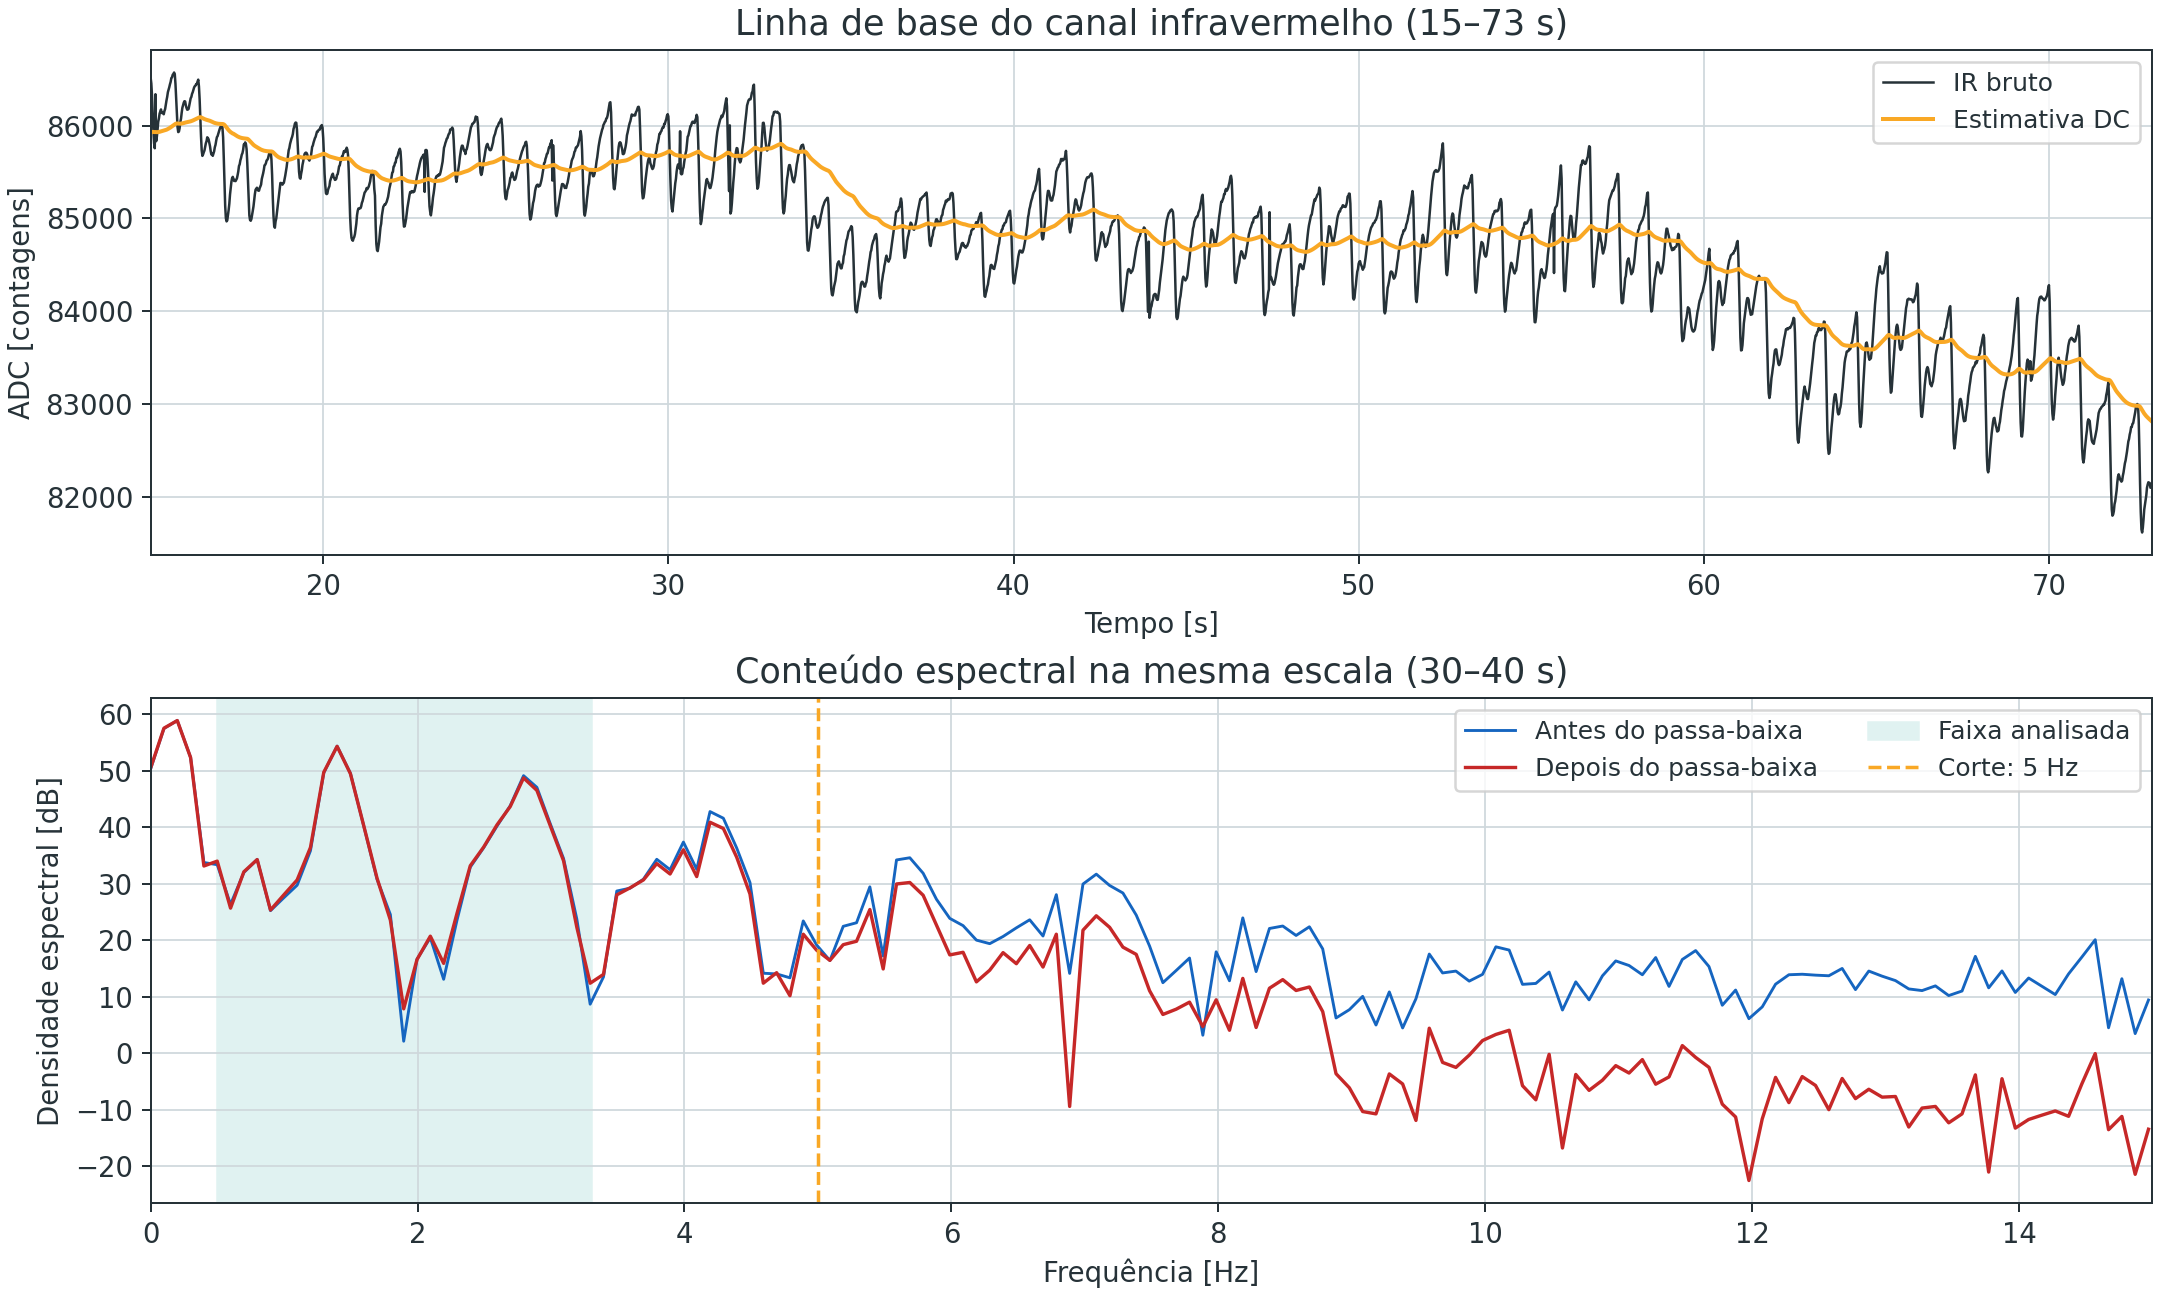
\includegraphics[width=0.98\textwidth]{Diagramas/max30102/max30102_ppg_condicionamento_15_73s.png}
\fonteelemento{Elaborado pelo autor a partir do CSV do ensaio standalone}
\end{figure}

O painel superior mostra a estimativa DC acompanhando a linha de base dominante do canal IR. O painel inferior confirma que a resposta antes e depois do passa-baixa permanece semelhante na faixa analisada e se separa progressivamente acima do corte de 5 Hz. N\~ao foi calculada rela\c{c}\~ao sinal-ru\'ido porque n\~ao havia trecho rotulado contendo somente ru\'ido sob a mesma condi\c{c}\~ao de contato. Tamb\'em n\~ao foi executada uma abla\c{c}\~ao do detector de batimentos com e sem o passa-baixa. Assim, os dados sustentam estima\c{c}\~ao de linha de base e limita\c{c}\~ao de banda, mas n\~ao demonstram que o passa-baixa tenha melhorado a exatid\~ao da frequ\^encia card\'iaca ou da SpO$_2$.


\subsubsection{Frequ\^encia card\'iaca e estimativa de SpO$_2$}

O teste standalone foi executado durante aproximadamente 65 s, com o ox\'imetro de dedo ECH e o Amazfit Active 2 operando simultaneamente. O ox\'imetro foi adotado como comparador principal. No primeiro trecho, ambos indicaram 81 BPM. Nas mudan\c{c}as seguintes, o MAX30102 acompanhou a dire\c{c}\~ao das cinco varia\c{c}\~oes observadas, mas apresentou subestima\c{c}\~ao em torno de 5 BPM nos patamares superiores, valores transit\'orios de 62 e 86 BPM e intervalos em estado de c\'alculo.

A SpO$_2$ do ox\'imetro permaneceu em 97\%, enquanto o MAX30102 indicou 98\% a 99\%. A diferen\c{c}a de 1 a 2 pontos percentuais e a estabilidade da indica\c{c}\~ao s\~ao compat\'iveis com um teste de plausibilidade, mas n\~ao constituem valida\c{c}\~ao cl\'inica. O ensaio foi realizado com um participante, instrumento de consumo sem certificado de calibra\c{c}\~ao e configura\c{c}\~ao standalone distinta da integra\c{c}\~ao final. A Figura~\ref{fig:fc-comparacao} sintetiza as indica\c{c}\~oes de frequ\^encia card\'iaca.

\begin{figure}[H]
\centering
\caption{Frequ\^encia card\'iaca indicada pelo MAX30102 e faixa observada no ox\'imetro}
\label{fig:fc-comparacao}
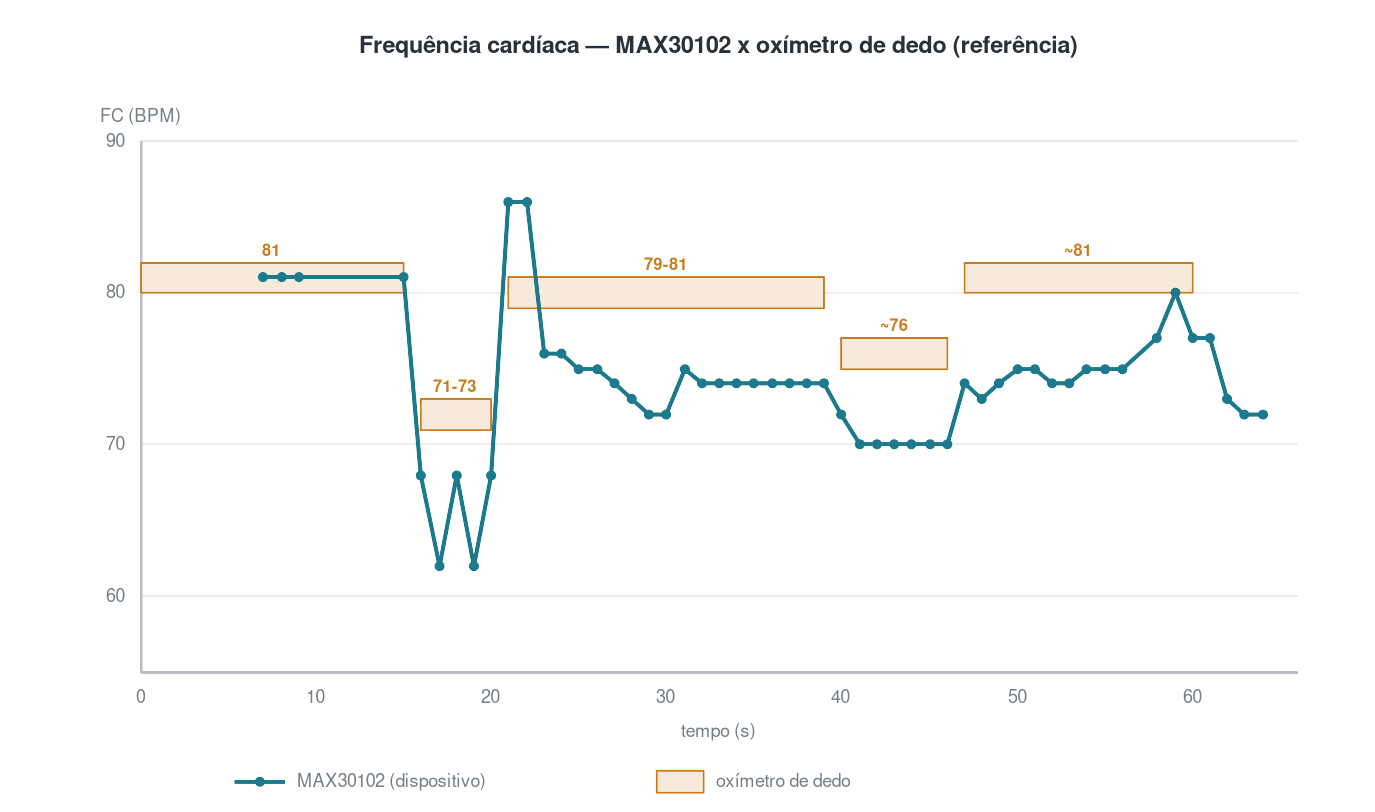
\includegraphics[width=0.95\textwidth]{Diagramas/max30102/max30102_fc_vs_referencia.png}
\fonteelemento{Elaborado pelo autor a partir do caderno de ensaios}
\end{figure}


A frequ\^encia card\'iaca e a SpO$_2$ permanecem resultados funcionais do pipeline. Movimento, contato, perfus\~ao, luz ambiente e posi\c{c}\~ao alteram a qualidade do PPG, e a calibra\c{c}\~ao emp\'irica empregada n\~ao transforma o prot\'otipo em instrumento cl\'inico.


\subsubsection{Evolu\c{c}\~ao das corre\c{c}\~oes}


A contribui\c{c}\~ao mais bem documentada do m\'odulo \'e a evolu\c{c}\~ao do processamento. A vers\~ao inicial produzia estimativas pr\'oximas de 70\%. A reorganiza\c{c}\~ao incluiu remo\c{c}\~ao de DC mais lenta, filtragem passa-baixa, detec\c{c}\~ao por batimento, per\'iodo refrat\'ario, raz\~ao calculada por ciclo e crit\'erios de qualidade.


Outro registro associa valores pr\'oximos de 28\% \`a troca dos canais vermelho e infravermelho em determinadas placas de conex\~ao; ap\'os corrigir a atribui\c{c}\~ao, foi observado valor pr\'oximo de 96\%. Essa observa\c{c}\~ao n\~ao deve ser generalizada ao MAX30102, mas evidencia a necessidade de conferir a ordem efetiva dos dados no m\'odulo utilizado.


As faixas de 70\%, 28\% e 95\%--99\% descrevem etapas de depura\c{c}\~ao, n\~ao um estudo comparativo. Como condi\c{c}\~oes e sinais correspondentes n\~ao est\~ao dispon\'iveis, elas n\~ao permitem separar o efeito individual de cada corre\c{c}\~ao.


\subsubsection{Limita\c{c}\~oes}


O per\'iodo refrat\'ario fixo de 400 ms imp\~oe limite te\'orico de 150 batimentos por minuto. O processamento n\~ao utiliza o aceler\^ometro para cancelar artefatos de movimento e emprega crit\'erios fixos de qualidade. A montagem em protoboard tamb\'em apresentou sensibilidade da alimenta\c{c}\~ao aos pulsos de corrente dos emissores.


\subsection{DS18B20}


\subsubsection{Estabilidade}

Durante aproximadamente 5 min, o DS18B20 permaneceu em 22,5 $^\circ$C e o termo-higr\^ometro MFL Embutir indicou 23,4 $^\circ$C. A diferen\c{c}a foi de $-0,9$ $^\circ$C. A toler\^ancia de $\pm0,5$ $^\circ$C informada para o DS18B20 n\~ao foi combinada a uma faixa do comparador, pois seu certificado e sua especifica\c{c}\~ao n\~ao estavam dispon\'iveis. Como a compara\c{c}\~ao ocorreu em um \`unico ponto, o resultado demonstra estabilidade de curto prazo e plausibilidade, n\~ao exatid\~ao metrol\'ogica. A figura anteriormente produzida com uma toler\^ancia ``t\'ipica'' assumida para o termo-higr\^ometro foi exclu\'ida desta vers\~ao.


\subsubsection{Resposta t\'ermica}

Partindo de 23 $^\circ$C, a leitura no freezer atingiu 13,4 $^\circ$C ap\'os 1 min e 3,3 $^\circ$C ap\'os 2 min. No aquecimento pr\'oximo \`a chama, a leitura atingiu 70 $^\circ$C em 30 s, quando o ensaio foi interrompido para preservar o probe. O intervalo observado foi de aproximadamente 67 $^\circ$C, sem travamento ou satura\c{c}\~ao. Como os est\'imulos n\~ao foram acompanhados por refer\^encia calibrada, os valores da Figura~\ref{fig:ds18b20-transientes} caracterizam resposta funcional e n\~ao acur\'acia din\^amica.

\begin{figure}[H]
\centering
\caption{Resposta do DS18B20 aos transientes de resfriamento e aquecimento}
\label{fig:ds18b20-transientes}
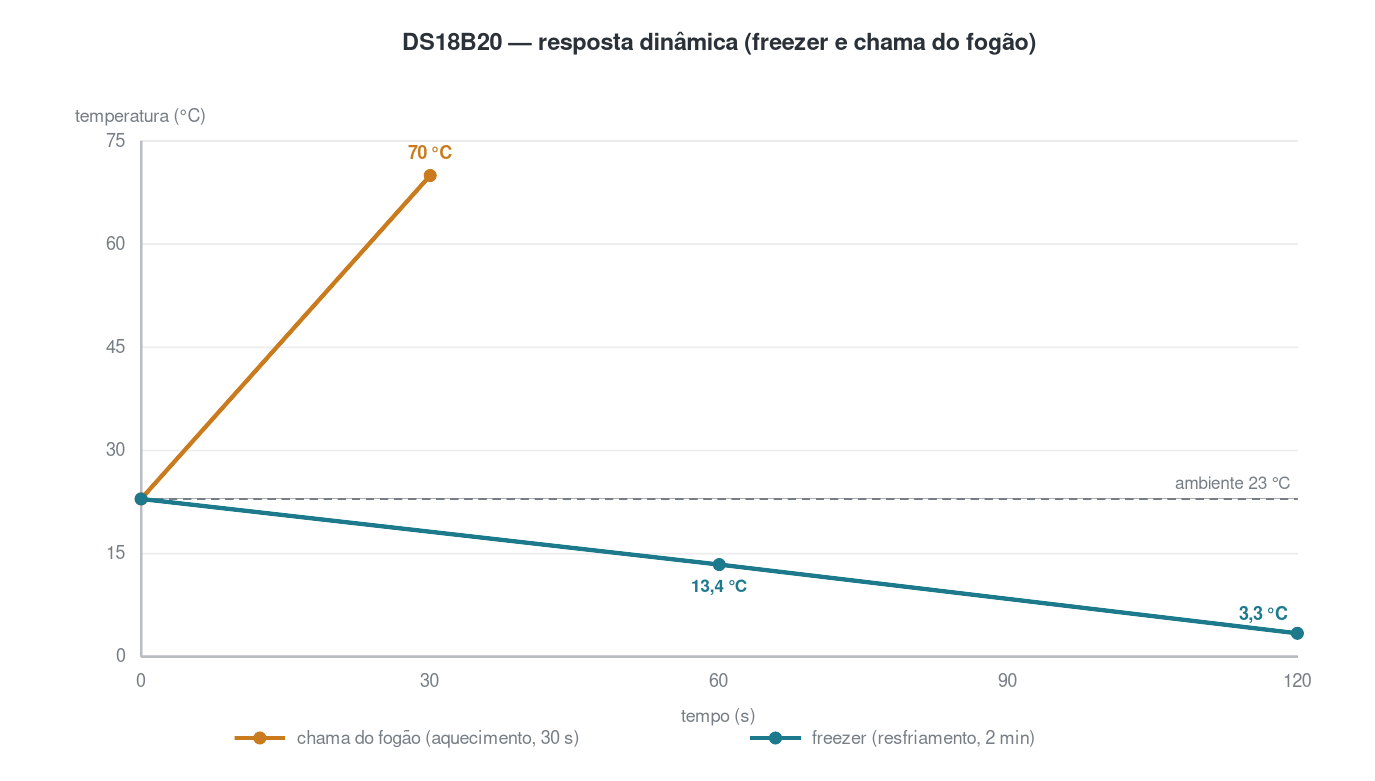
\includegraphics[width=0.85\textwidth]{Diagramas/ds18b20/ds18b20_resposta_dinamica.png}
\fonteelemento{Elaborado pelo autor a partir do caderno de ensaios}
\end{figure}


\subsubsection{Limita\c{c}\~oes}


A leitura depende da posi\c{c}\~ao, da transfer\^encia t\'ermica pela montagem e das fontes de calor pr\'oximas. Repeti\c{c}\~ao de um valor digital n\~ao deve ser interpretada como exatid\~ao.


\subsection{LTR390}


\subsubsection{Ambiente interno}


O compilado registra contagens entre 185 e 188 no canal ALS, correspondentes a aproximadamente 37,0--37,6 lux pela convers\~ao adotada. No mesmo ambiente, com ilumina\c{c}\~ao LED e janelas fechadas, o canal UVS permaneceu em zero.


A baixa varia\c{c}\~ao demonstra repetibilidade de curto prazo das contagens naquele cen\'ario, mas n\~ao exatid\~ao em lux. O valor nulo no canal UV \'e fisicamente plaus\'ivel em ambiente sem fonte ultravioleta relevante, embora n\~ao demonstre sensibilidade do canal a uma exposi\c{c}\~ao conhecida.


\subsubsection{Ensaio externo de UVI}


O resumo consolidado cita ensaio ao ar livre em Florian\'opolis no qual a estimativa variou entre UVI 3 e 6, com pico 6, enquanto uma refer\^encia meteorol\'ogica indicava UVI 5.


O registro indica resposta do sensor \`a radia\c{c}\~ao solar e compatibilidade de ordem de grandeza com a refer\^encia. N\~ao constitui calibra\c{c}\~ao, pois a refer\^encia meteorol\'ogica n\~ao foi medida junto ao sensor e pode representar intervalo espacial e temporal diferente.


O ensaio ocorreu em 25 de julho de 2026, em Florian\'opolis, sob c\'eu limpo. A aus\^encia de difusor cosseno e a movimenta\c{c}\~ao manual do prot\'otipo limitaram o controle angular. Em teste standalone adicional, uma lanterna UV gen\'erica elevou a indica\c{c}\~ao de 0 at\'e aproximadamente 4,0 conforme foi aproximada de 20 cm at\'e muito perto do sensor. Esse segundo ensaio confirma resposta qualitativa do canal, mas a fonte n\~ao caracterizada n\~ao fornece refer\^encia de UVI. A Figura~\ref{fig:ltr390-uvi} posiciona a faixa observada apenas para compara\c{c}\~ao qualitativa.

\begin{figure}[H]
\centering
\caption{Faixa de UVI indicada pelo LTR390 e valor meteorol\'ogico de refer\^encia}
\label{fig:ltr390-uvi}
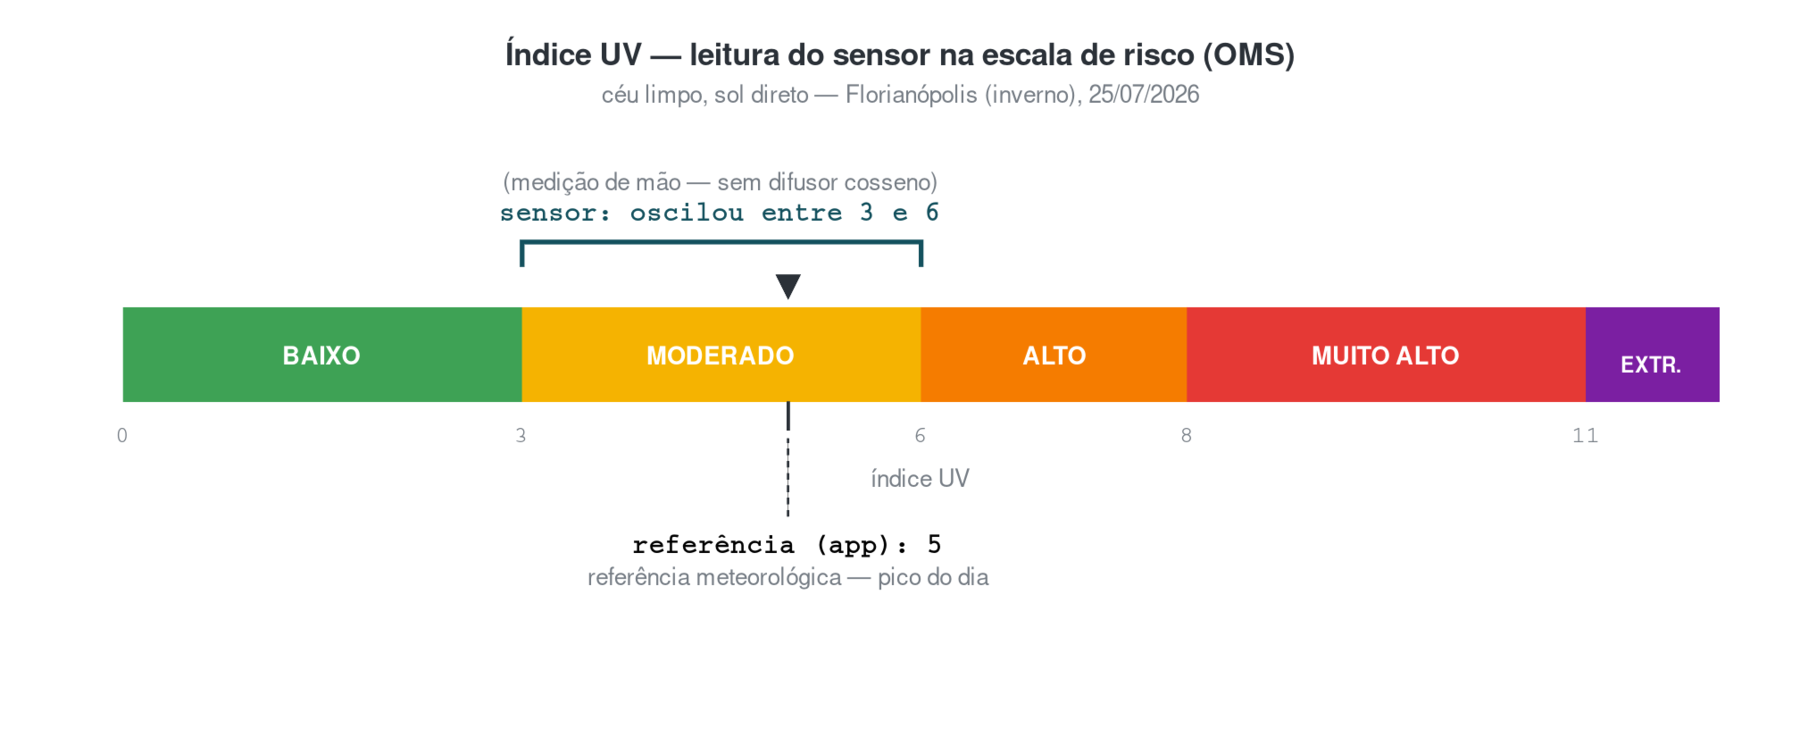
\includegraphics[width=0.8\textwidth]{Diagramas/ltr390/ltr390_uv_escala_risco.png}
\fonteelemento{Elaborado pelo autor a partir do caderno de ensaios e da refer\^encia meteorol\'ogica consultada}
\end{figure}


\subsubsection{Faixa e satura\c{c}\~ao de ilumin\^ancia}


O mesmo resumo informa resposta desde obstru\c{c}\~ao at\'e aproximadamente 52 klux e satura\c{c}\~ao pr\'oxima desse valor na configura\c{c}\~ao de ganho 3$\times$ e 18 bits. A satura\c{c}\~ao deve ser atribu\'ida \`a configura\c{c}\~ao usada, n\~ao ao limite absoluto do LTR390.


Foram observados 0 lux no escuro, aproximadamente 10--30 lux sob ilumina\c{c}\~ao urbana noturna, 100--150 lux em ambiente interno, cerca de 4000 lux em sombra externa e 51--52 klux sob sol direto. O \`ultimo valor coincide com o teto calculado de aproximadamente 52,4 klux para ganho 3$\times$ e resolu\c{c}\~ao de 18 bits, indicando satura\c{c}\~ao da configura\c{c}\~ao, n\~ao necessariamente da faixa absoluta do sensor. A Figura~\ref{fig:ltr390-lux} usa escala logar\'itmica para reunir essas ordens de grandeza.

\begin{figure}[H]
\centering
\caption{Ilumin\^ancia observada e teto da configura\c{c}\~ao utilizada}
\label{fig:ltr390-lux}
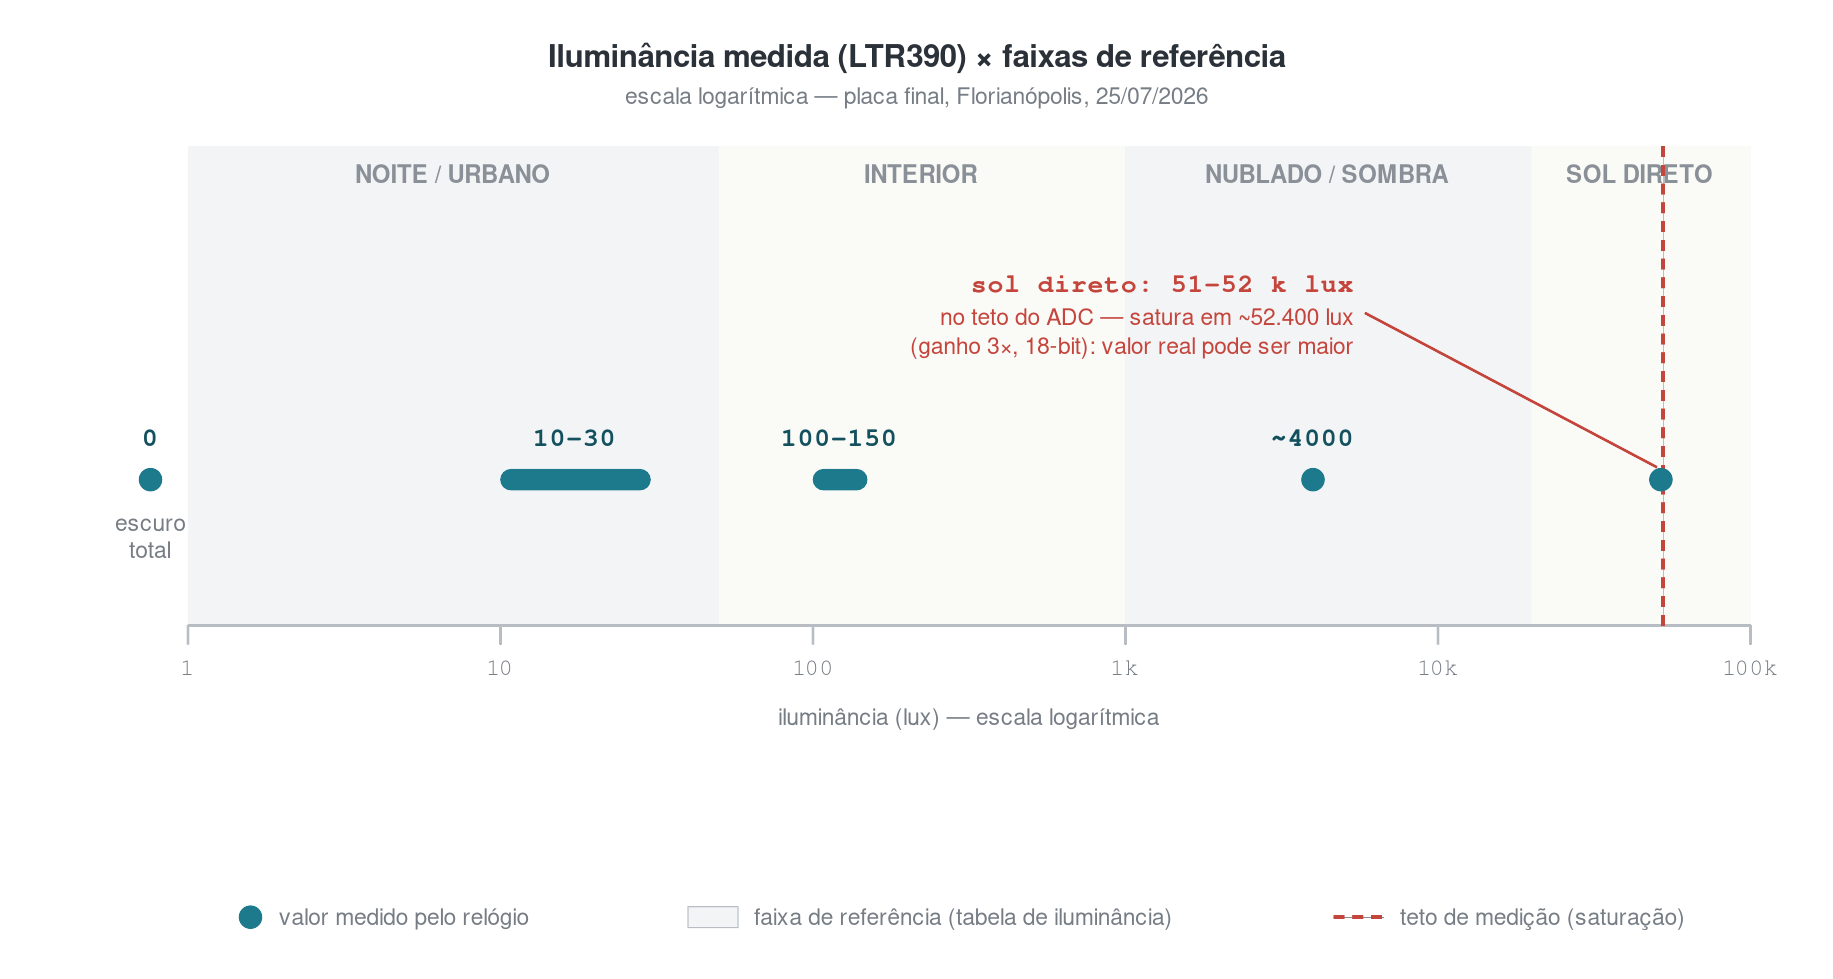
\includegraphics[width=0.85\textwidth]{Diagramas/ltr390/ltr390_lux_escala_log.png}
\fonteelemento{Elaborado pelo autor a partir do caderno de ensaios}
\end{figure}


\subsubsection{Limita\c{c}\~oes}


ALS e UVS n\~ao s\~ao medidos simultaneamente. A altern\^ancia introduz intervalo de estabiliza\c{c}\~ao e mant\'em cada valor at\'e a pr\'oxima ativa\c{c}\~ao do canal. Janela \'optica, orienta\c{c}\~ao, sombra e espectro da fonte afetam as leituras.


\subsection{B\'ussola}


\subsubsection{Calibra\c{c}\~ao}


A calibra\c{c}\~ao no pr\'oprio dispositivo, dividida em 12 setores e persistida em NVS, substituiu o fluxo anterior de exporta\c{c}\~ao CSV. A divis\~ao em setores orienta a coleta, mas a calibra\c{c}\~ao diagonal n\~ao corrige termos cruzados de \emph{soft iron}.


N\~ao foi preservada uma nuvem de pontos antes e depois da calibra\c{c}\~ao nem o conjunto final de par\^ametros usado no ensaio. Assim, a centraliza\c{c}\~ao, as diferen\c{c}\~as de escala e a cobertura tridimensional n\~ao foram quantificadas. A figura conceitual apresentada na Fundamenta\c{c}\~ao explica o m\'etodo, mas n\~ao foi reutilizada aqui como se fosse resultado do prot\'otipo.


\subsubsection{Heading}

Com o prot\'otipo e a b\'ussola Norvix DC45-2 nivelados no mesmo plano, foram comparadas duas orienta\c{c}\~oes na vers\~ao de ensaio, que n\~ao aplicava ajuste de declina\c{c}\~ao. Na ida, a Norvix indicou 320$^\circ$ e o prot\'otipo 336$^\circ$, diferen\c{c}a de +16$^\circ$. Na volta, as indica\c{c}\~oes foram 130$^\circ$ e 152$^\circ$, diferen\c{c}a de +22$^\circ$. A diferen\c{c}a m\'edia assinada foi +19$^\circ$.

Como ambos os instrumentos indicavam norte magn\'etico, o deslocamento n\~ao pode ser atribu\'ido \`a declina\c{c}\~ao. Calibra\c{c}\~ao residual, alinhamento visual, interfer\^encia da montagem e diferen\c{c}a entre os instrumentos s\~ao explica\c{c}\~oes poss\'iveis, mas n\~ao separadas pelo procedimento. O ensaio confirma resposta direcional, mas n\~ao sustenta alega\c{c}\~ao de precis\~ao. A Figura~\ref{fig:bussola-comparacao} identifica explicitamente a vers\~ao magn\'etica avaliada.


\begin{figure}[H]
\centering
\caption{Compara\c{c}\~ao magn\'etica entre o prot\'otipo e a b\'ussola de consumo}
\label{fig:bussola-comparacao}
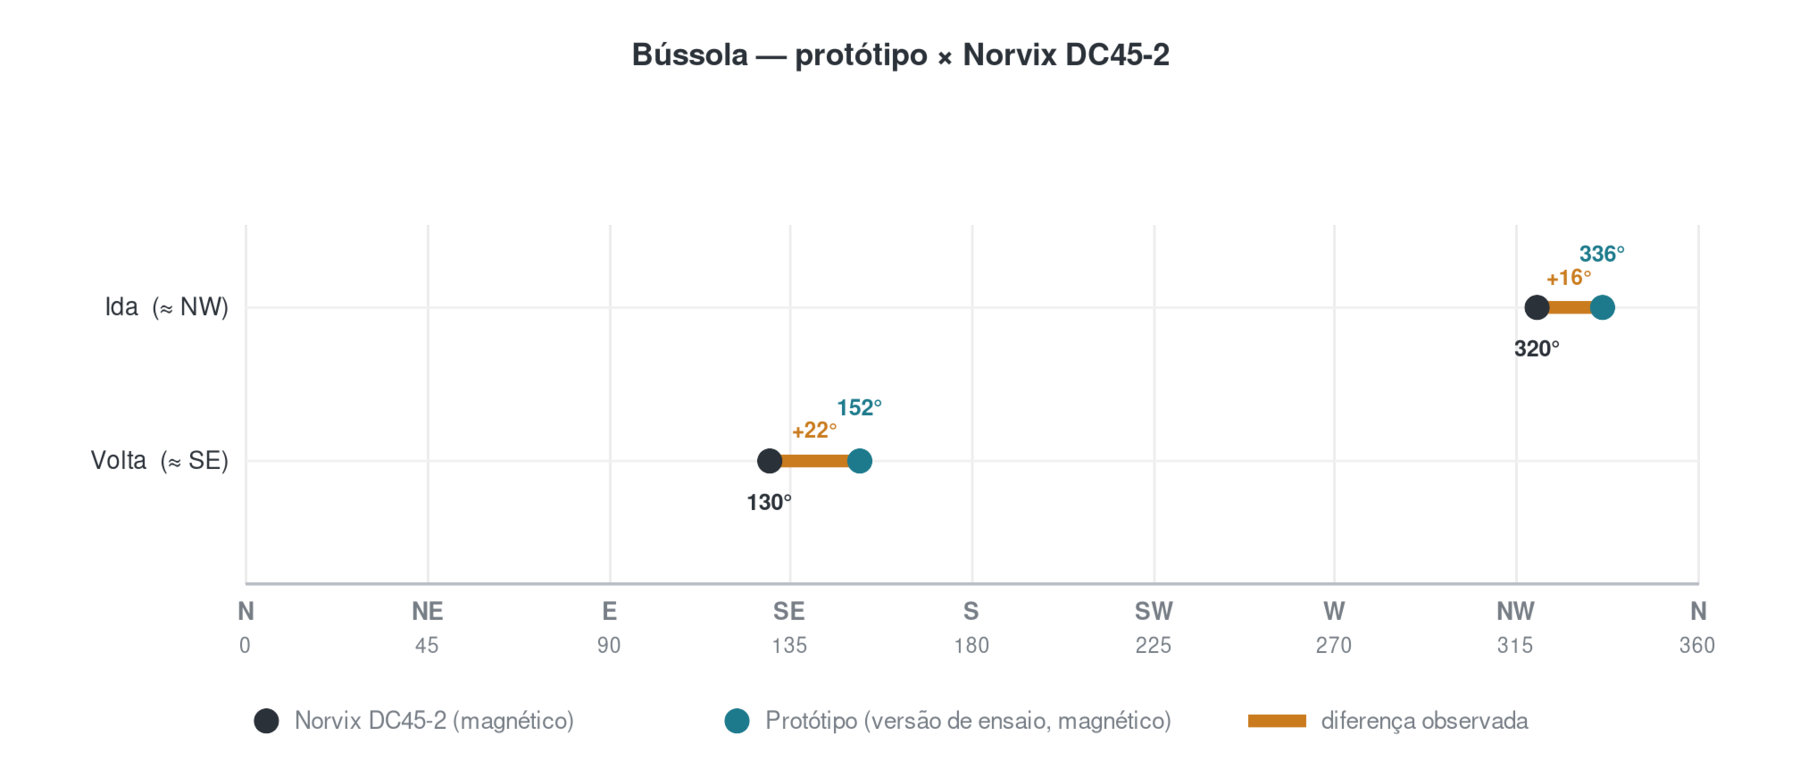
\includegraphics[width=0.95\textwidth]{Diagramas/mpu9250/mpu9250_bussola_declinacao.png}
\fonteelemento{Elaborado pelo autor a partir do caderno de ensaios}
\end{figure}


\subsubsection{Limita\c{c}\~oes}


Os valores do ensaio referem-se ao norte magn\'etico porque a vers\~ao avaliada n\~ao aplicava declina\c{c}\~ao. O firmware corrente acrescenta um valor fixo de $-21^\circ$; essa altera\c{c}\~ao posterior n\~ao deve ser usada para reinterpretar retroativamente as medidas. Inclina\c{c}\~ao do dispositivo projeta a componente vertical do campo nos eixos do c\'alculo, e a compensa\c{c}\~ao correspondente n\~ao foi implementada. Materiais ferromagn\'eticos e correntes do prot\'otipo podem alterar a calibra\c{c}\~ao.


\subsection{Ped\^ometro}


\subsubsection{Teste qualitativo}


O compilado descreve balan\c{c}o manual da protoboard e uma simula\c{c}\~ao com o sensor preso \`a perna. Foram relatadas detec\c{c}\~oes durante movimento, aus\^encia de falsos positivos em repouso e correspond\^encia considerada razo\'avel com os passos executados.


N\~ao foram informados n\'umero de passos, dura\c{c}\~ao do repouso, ritmo, posi\c{c}\~ao exata, repeti\c{c}\~oes nem erros. O registro confirma que o algoritmo responde a oscila\c{c}\~oes, mas n\~ao caracteriza seu desempenho como ped\^ometro.


\subsubsection{Ensaio controlado}

Em percurso de 100 m delimitado no Google Maps, a contagem manual foi de 140 passos tanto na ida quanto na volta. O prot\'otipo registrou 131 e 133 passos, correspondentes a erros de $-6,4$\% e $-5,0$\%, com m\'edia de $-5,7$\%. O Amazfit Active 2 registrou 175 e 167 passos, erros de +25,0\% e +19,3\%. A diferen\c{c}a entre as duas repeti\c{c}\~oes foi de 2 passos no prot\'otipo e 8 no comparador comercial. A Tabela~\ref{tab:pedometro-100m} organiza os valores observados.

\begin{table}[H]
\centering
\caption{Contagens e erros observados no percurso de 100 m}
\label{tab:pedometro-100m}
\begin{tabular}{lrrrrr}
\toprule
Percurso & Manual & Prot\'otipo & Erro (\%) & Amazfit & Erro (\%) \\
\midrule
Ida   & 140 & 131 & $-6,4$ & 175 & $+25,0$ \\
Volta & 140 & 133 & $-5,0$ & 167 & $+19,3$ \\
\bottomrule
\end{tabular}
\fonteelemento{Elaborado pelo autor a partir do caderno de ensaios}
\end{table}

O resultado indica subestima\c{c}\~ao moderada e pequena varia\c{c}\~ao entre os dois percursos nas condi\c{c}\~oes observadas. Entretanto, limita-se a um participante, um ritmo e duas repeti\c{c}\~oes. A dist\^ancia m\'edia por passo calculada pela refer\^encia foi 0,714 m, pr\'oxima do valor fixo de 0,70 m empregado pelo firmware. A Figura~\ref{fig:pedometro-ensaio} preserva as contagens de cada percurso.

\begin{figure}[H]
\centering
\caption{Contagem manual, prot\'otipo e Amazfit Active 2 no percurso de 100 m}
\label{fig:pedometro-ensaio}
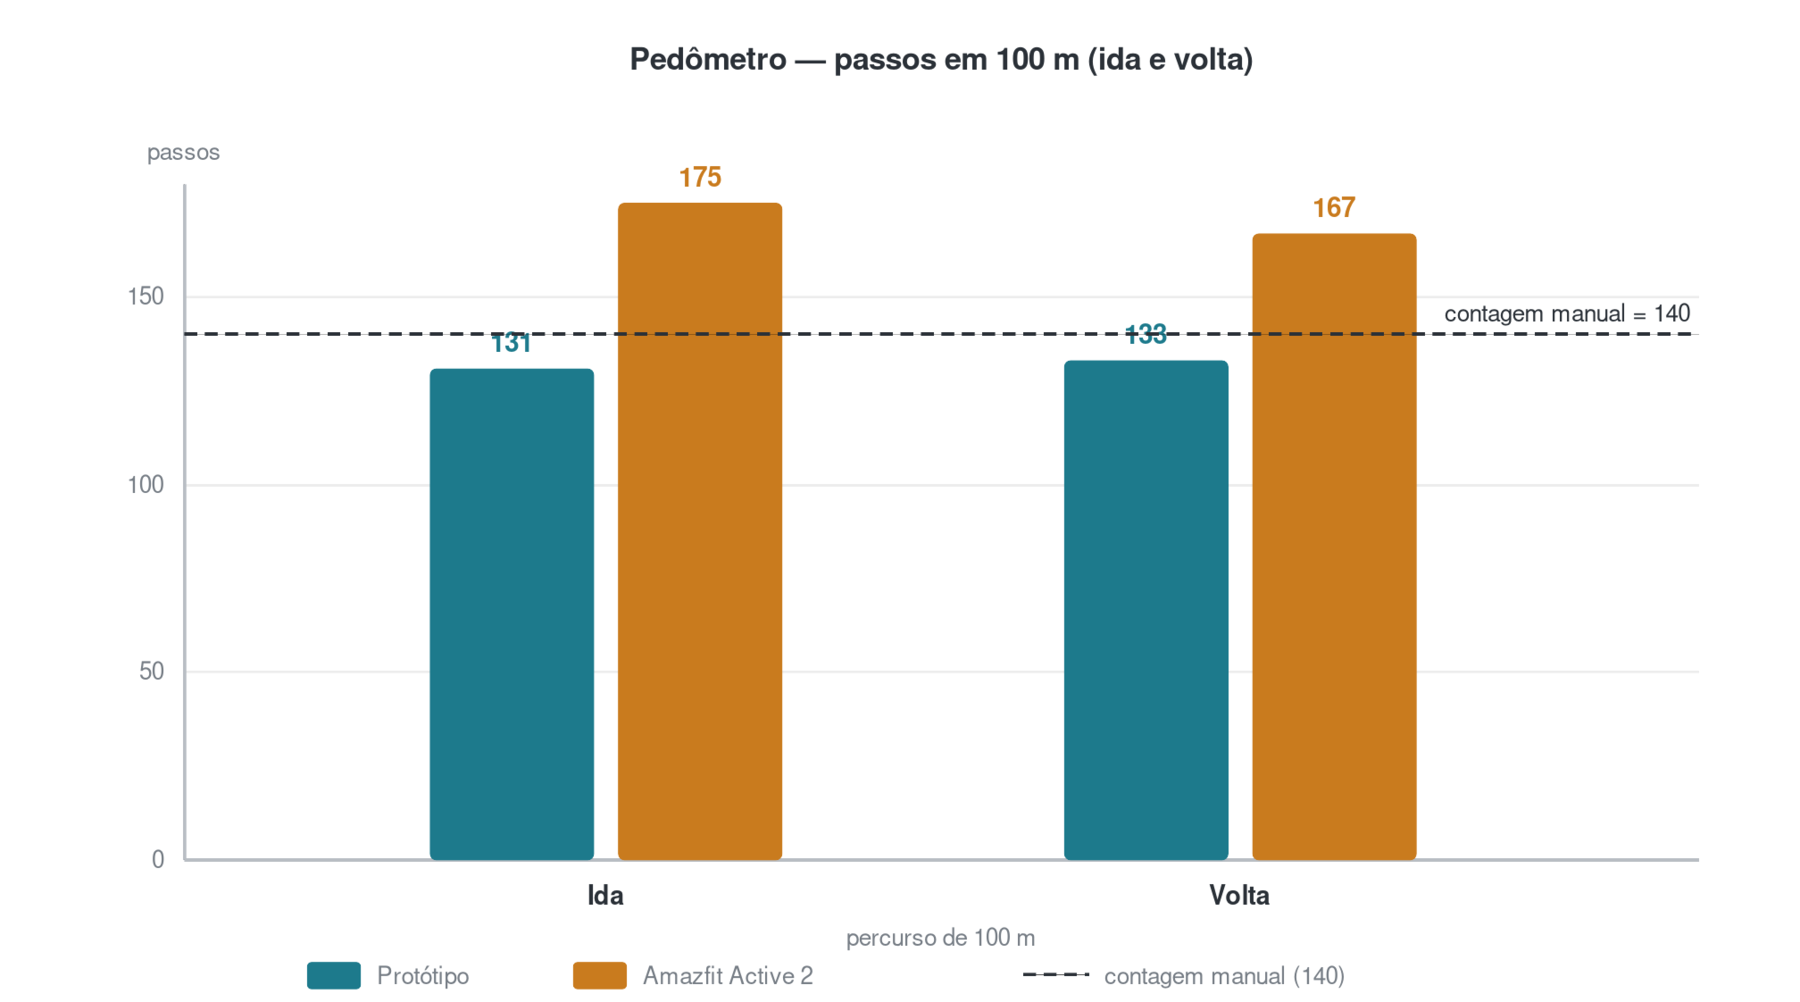
\includegraphics[width=0.85\textwidth]{Diagramas/mpu9250/mpu9250_pedometro_passos.png}
\fonteelemento{Elaborado pelo autor a partir do caderno de ensaios}
\end{figure}


\subsubsection{Limita\c{c}\~oes}


Limiar, histerese e intervalo m\'inimo s\~ao fixos. Movimentos do bra\c{c}o ou do dispositivo podem produzir cruzamentos semelhantes aos da marcha, enquanto passos suaves podem n\~ao atingir o limiar. A dist\^ancia usa comprimento fixo de 0,70 m e n\~ao foi individualizada. O contador retorna a zero ap\'os reinicializa\c{c}\~ao.


\subsection{Interface gr\'afica}


Os compilados registram funcionamento da exibi\c{c}\~ao de hora e data, anel de segundos, edi\c{c}\~ao por toque, grava\c{c}\~ao no PCF8563 e navega\c{c}\~ao entre as fun\c{c}\~oes. A calibra\c{c}\~ao da b\'ussola e o in\'icio da aquisi\c{c}\~ao PPG tamb\'em utilizam controles gr\'aficos.


A identifica\c{c}\~ao do CHSC6X por varredura em 0x2E permitiu substituir o driver inicialmente escolhido com base na documenta\c{c}\~ao de outra revis\~ao. A fonte restrita a 11 glifos reduziu armazenamento e exigiu que o feedback da edi\c{c}\~ao fosse implementado por opacidade.


Esses resultados demonstram integra\c{c}\~ao funcional entre toque, RTC, LVGL e m\'odulos. As capturas da Figura~\ref{fig:interface-final} pertencem \`a mesma sequ\^encia registrada no firmware corrente e documentam a tela principal, as quatro p\'aginas de menu por meio de exemplos representativos e telas funcionais.


\begin{figure}[H]
\centering
\caption{Capturas da interface execut\'avel da plataforma}
\label{fig:interface-final}
\begin{subfigure}[t]{0.26\textwidth}
\centering
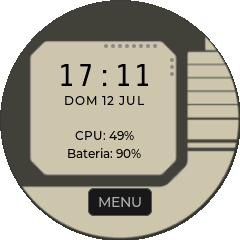
\includegraphics[width=\linewidth]{Telas Display/tela_230002_01_MenuPrincipal.png}
\caption{Tela principal}
\end{subfigure}
\hfill
\begin{subfigure}[t]{0.26\textwidth}
\centering
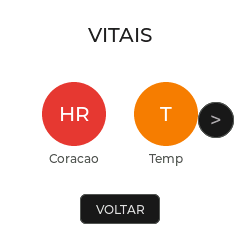
\includegraphics[width=\linewidth]{Telas Display/tela_230024_02_VitaisMenu.png}
\caption{Sinais vitais}
\end{subfigure}
\hfill
\begin{subfigure}[t]{0.26\textwidth}
\centering
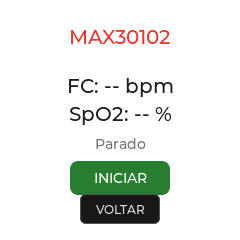
\includegraphics[width=\linewidth]{Telas Display/tela_230056_03_MaxScreen.png}
\caption{PPG}
\end{subfigure}

\medskip
\begin{subfigure}[t]{0.26\textwidth}
\centering
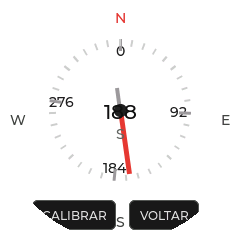
\includegraphics[width=\linewidth]{Telas Display/tela_230333_09_CompScreen.png}
\caption{B\'ussola}
\end{subfigure}
\hfill
\begin{subfigure}[t]{0.26\textwidth}
\centering
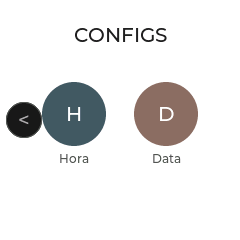
\includegraphics[width=\linewidth]{Telas Display/tela_230412_11_ConfigMenu.png}
\caption{Configura\c{c}\~oes}
\end{subfigure}
\hfill
\begin{subfigure}[t]{0.26\textwidth}
\centering
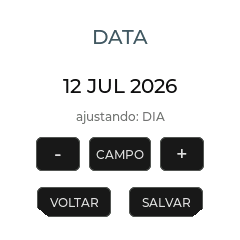
\includegraphics[width=\linewidth]{Telas Display/tela_230505_13_DataScreen.png}
\caption{Ajuste de data}
\end{subfigure}
\begin{minipage}{0.92\textwidth}
\fonteelemento{Capturas do firmware integrado produzidas pelo autor}
\end{minipage}
\end{figure}

No ensaio do RTC, a hora foi ajustada na troca de minuto da refer\^encia oficial de Bras\'ilia. Depois de 1 h com o sistema ligado, n\~ao foi observado desvio na resolu\c{c}\~ao do procedimento. Em seguida, o sistema permaneceu desligado por 24 h; ao religar, o PCF8563 apresentou atraso de aproximadamente 2 s. O resultado demonstra que a bateria CR927 preservou a contagem durante o desligamento. A observa\c{c}\~ao de um \`unico intervalo de 24 h corresponde a cerca de 2 s/dia ou 23 ppm, mas n\~ao substitui caracteriza\c{c}\~ao de deriva por v\'arios dias. A sequ\^encia \'e sintetizada na Figura~\ref{fig:rtc-sequencia}.

\begin{figure}[H]
\centering
\caption{Sequ\^encia do ensaio de manuten\c{c}\~ao da hora com o sistema desligado}
\label{fig:rtc-sequencia}
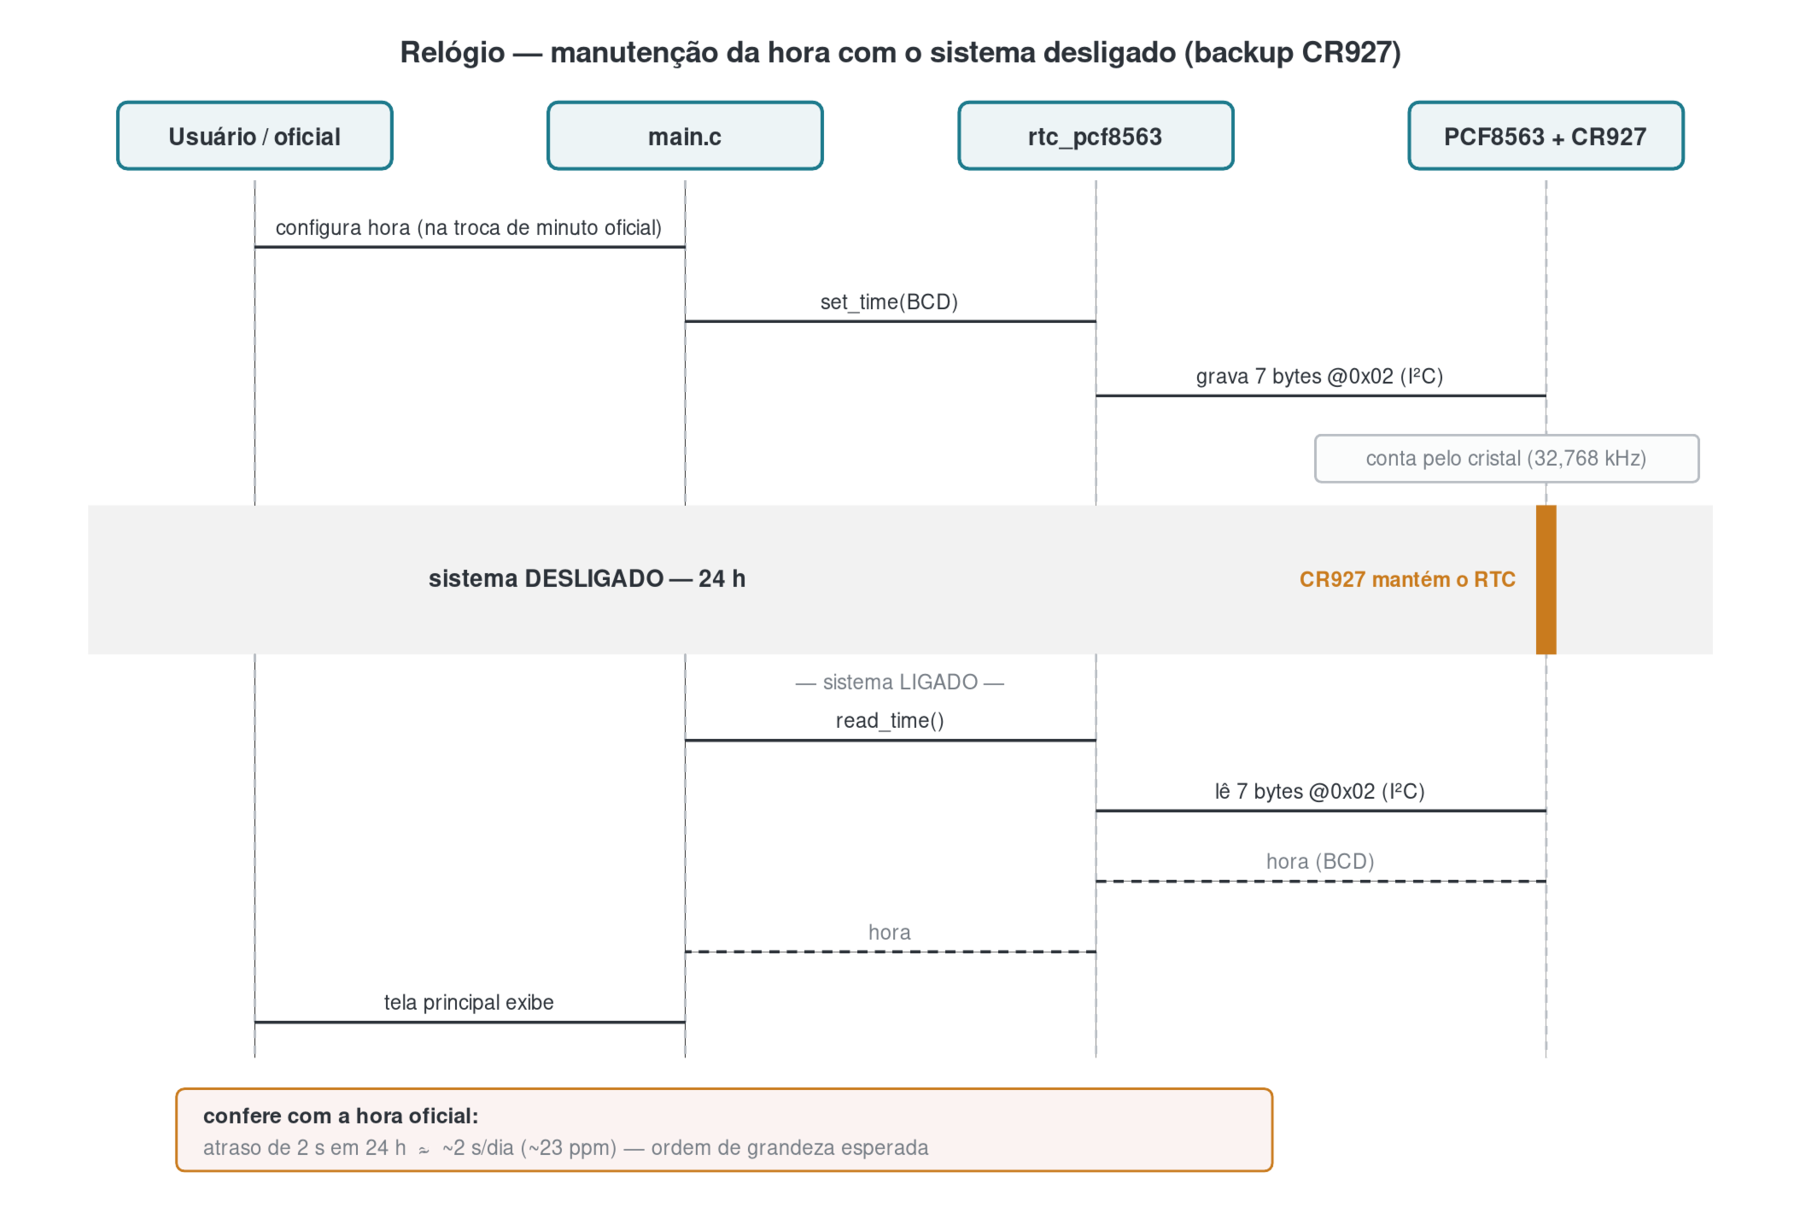
\includegraphics[width=0.95\textwidth]{Diagramas/round_display/relogio_rtc_sequencia.png}
\fonteelemento{Elaborado pelo autor a partir do caderno de ensaios}
\end{figure}


As capturas confirmam composi\c{c}\~ao e navegabilidade das telas mostradas, mas n\~ao medem lat\^encia nem taxa de falhas de toque. Essas m\'etricas n\~ao foram coletadas.


\subsection{Alimenta\c{c}\~ao e bateria}


O resumo consolidado registra leituras pontuais de aproximadamente 4,04 V com USB conectado e 3,84 V somente com bateria, associadas pelo firmware a 88\% e 56\%. Com USB, a tens\~ao observada pertence ao estado de carga e n\~ao representa a curva de descarga da c\'elula.


Essas leituras n\~ao sustentam autonomia, capacidade efetiva ou estado de carga com a exatid\~ao indicada pelos percentuais. O backlight permanece ligado e o gerenciamento avan\c{c}ado de energia n\~ao foi implementado.

O mult\'imetro foi ligado em s\'erie com a bateria para medir nove cen\'arios. A tela principal consumiu 110 mA; menu, 120 mA; temperatura, 150 mA; luz/UV, 130 mA; b\'ussola, 180 mA; calibra\c{c}\~ao da b\'ussola, 130 mA; ped\^ometro, 120 mA; tela PPG parada, 90 mA; e PPG medindo, 210 mA. As associa\c{c}\~oes entre essas diferen\c{c}as e atividades espec\'ificas de CPU, interface ou sensores s\~ao hip\'oteses a confirmar, pois o ensaio mediu somente a corrente total.

N\~ao foi executada descarga completa. Com capacidade \`util assumida de aproximadamente 1000 mAh, a raz\~ao entre capacidade e corrente fornece estimativas de autonomia dependentes do cen\'ario; elas n\~ao constituem autonomia medida. O backlight permaneceu ligado e os modos de baixo consumo foram tratados como proje\c{c}\~ao de trabalho futuro. A Figura~\ref{fig:consumo-cenarios} apresenta apenas as correntes totais observadas.

\begin{figure}[H]
\centering
\caption{Corrente total medida nos cen\'arios funcionais da plataforma}
\label{fig:consumo-cenarios}
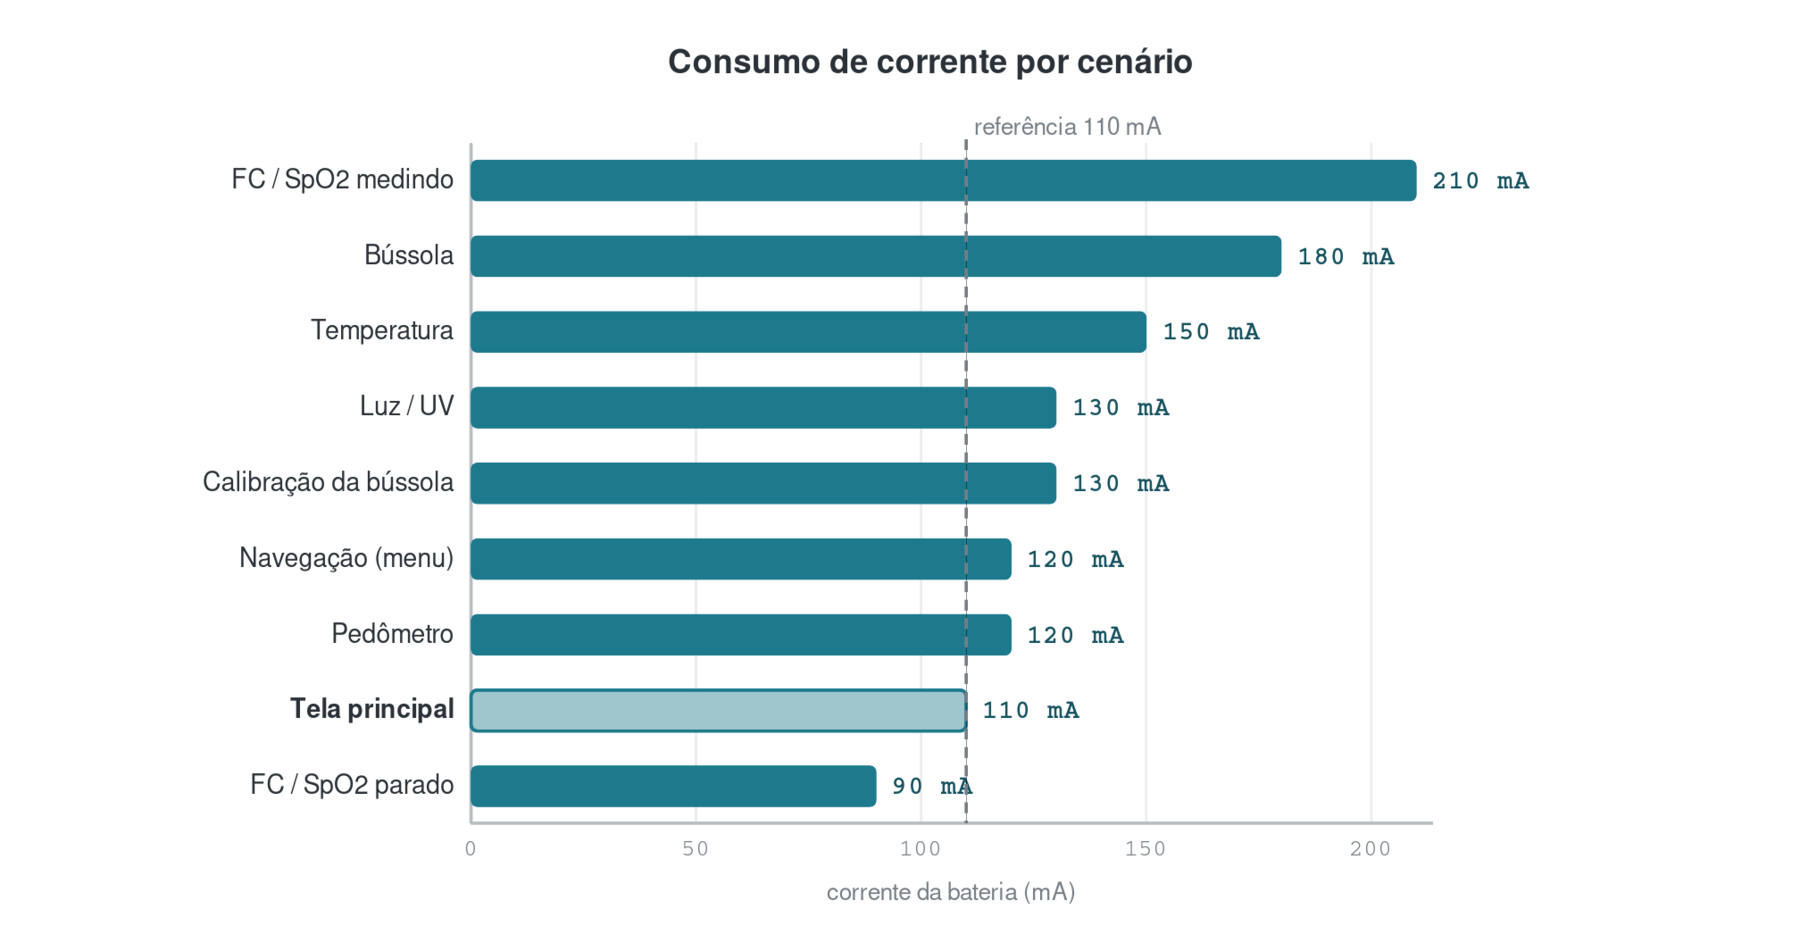
\includegraphics[width=0.85\textwidth]{Diagramas/bateria/bateria_consumo_por_cenario.png}
\fonteelemento{Elaborado pelo autor a partir do caderno de ensaios}
\end{figure}


\subsection{Discuss\~ao integrada}


A integra\c{c}\~ao funcional \'e a evid\^encia mais consistente do estado atual. O mesmo n\'ucleo organiza interface, RTC e quatro unidades sensoriais, apesar de diferen\c{c}as de transporte, per\'iodo e processamento. O contrato de m\'odulos, o registro de telas e as tarefas independentes materializam as caracter\'isticas de modularidade e extensibilidade descritas no projeto.


O barramento I$^2$C concentrou os principais efeitos sist\^emicos. \emph{Polling} excessivo do toque, NACK do LTR390 durante reset e verbosidade dos logs deixaram de ser problemas confinados aos respectivos drivers porque disputavam controlador, CPU e tempo de execu\c{c}\~ao. As corre\c{c}\~oes --- interrup\c{c}\~ao do toque, remo\c{c}\~ao do reset desnecess\'ario, mutex e recupera\c{c}\~ao --- mostram que a robustez depende da coordena\c{c}\~ao dos servi\c{c}os compartilhados.


Os ensaios com sensores ausentes complementam a an\'alise estrutural: a remo\c{c}\~ao individual de cada sensor e os diferentes arranjos de remo\c{c}\~ao n\~ao impediram a opera\c{c}\~ao do sistema principal nem dos m\'odulos independentes. Como a falha din\^amica do barramento n\~ao foi induzida e n\~ao se estabeleceu um protocolo estat\'istico de repeti\c{c}\~oes, essa rela\c{c}\~ao comprova a conten\c{c}\~ao funcional nas condi\c{c}\~oes testadas, mas n\~ao define uma taxa de confiabilidade.


Nos m\'odulos sensoriais, as evid\^encias possuem car\'ater funcional. O PPG foi comparado com ox\'imetro de consumo sem valida\c{c}\~ao cl\'inica; o DS18B20 foi comparado em um ponto com refer\^encia n\~ao calibrada; a compara\c{c}\~ao meteorol\'ogica do LTR390 n\~ao \'e calibra\c{c}\~ao; a b\'ussola apresentou diferen\c{c}as de 16$^\circ$ e 22$^\circ$ em apenas duas orienta\c{c}\~oes; e o ped\^ometro foi ensaiado com um participante, um ritmo e duas repeti\c{c}\~oes. Essa delimita\c{c}\~ao evita converter plausibilidade em valida\c{c}\~ao.


\subsection{Compara\c{c}\~ao com trabalhos relacionados}


O Amulet avalia uma plataforma para m\'ultiplas aplica\c{c}\~oes com \^enfase em energia, isolamento e acesso a recursos (HESTER et al., 2016). A WMP concentra-se na aquisi\c{c}\~ao sincronizada de sinais fisiol\'ogicos e em processamento remoto (BALDINI et al., 2023). O WEARDA prioriza coleta aberta e reprodut\'ivel de dados em um smartwatch comercial (VAN DIJK; GAWEHNS; VAN LEEUWEN, 2023).


O presente trabalho concentra-se no firmware de uma plataforma vest\'ivel modular multissensor constru\'ida sobre microcontrolador e sensores heterog\^eneos. Seu diferencial proposto est\'a no contrato de m\'odulos, na coordena\c{c}\~ao expl\'icita do I$^2$C compartilhado e na continuidade das fun\c{c}\~oes independentes quando um sensor est\'a ausente. Amulet e WMP apresentam avalia\c{c}\~oes experimentais mais estruturadas em seus respectivos objetivos.


A compara\c{c}\~ao n\~ao estabelece superioridade geral. Cada plataforma adota escopo, hardware e unidade de an\'alise diferentes, e as m\'etricas dispon\'iveis n\~ao permitem uma classifica\c{c}\~ao \'unica.


\subsection{Limita\c{c}\~oes gerais}


A placa prot\'otipo e o inv\'olucro impresso em 3D foram realizados, mas n\~ao passaram por caracteriza\c{c}\~ao mec\^anica, ambiental ou de uso prolongado. O backlight sempre ligado e a aus\^encia de gerenciamento avan\c{c}ado de energia limitam a autonomia; como n\~ao houve descarga completa, somente estimativas derivadas do consumo medido podem ser apresentadas.


N\~ao houve valida\c{c}\~ao cl\'inica do MAX30102, calibra\c{c}\~ao metrol\'ogica do LTR390, caracteriza\c{c}\~ao t\'ermica com refer\^encia rastre\'avel, compensa\c{c}\~ao de inclina\c{c}\~ao da b\'ussola nem caracteriza\c{c}\~ao estat\'istica do ped\^ometro para diferentes usu\'arios e ritmos.


Tamb\'em permaneceram fora do escopo a carga de CPU e o heap por cen\'ario, a mem\'oria incremental por m\'odulo, uma s\'erie controlada de tempo de boot, a recupera\c{c}\~ao I$^2$C sob falhas induzidas e um ensaio prolongado com navega\c{c}\~ao repet\'ivel.

\end{document}
